%%%%%%%%%%%%%%%%%%%%%%%%%%%%%%%%%%%%%%%%%%%%%%%%%%%%%%%%%%%%%%%%%%%%%%%%%%%%%%%%
% Preámbulo                                                                    %
%%%%%%%%%%%%%%%%%%%%%%%%%%%%%%%%%%%%%%%%%%%%%%%%%%%%%%%%%%%%%%%%%%%%%%%%%%%%%%%%

\documentclass[11pt,a4paper,titlepage,oneside]{report}

%%% RELACIÓN DE VARIABLES A PERSONALIZAR %%%
\def\lingua{esp}
\def\nome{Pablo Rey Ansemil}                             % substitúe aquí o teu nome
\def\nomedirectorA{María José Martín Santamaría}         % substitúe aquí o nome de quen dirixe
\def\nomedirectorB{Jorge González Domínguez}             % duplica esta liña máis veces se o precisas, cambiando
                                                     % a letra final (A, B, C, D...): úsanse na portada.tex
\def\titulo{Modelado en tiempo de la dispersión estelar de la vía láctea utilizando infraestructuras de altas prestaciones} % substitúe aquí o título do teu TFG
%\def\titulacion{gced}                               % descomenta esta liña e comenta a seguinte se es estudante do GCED
\def\titulacion{gei}
%\def\mencion{COMPUTACIÓN}                           % descomenta a mención que che corresponda se es estudante do GEI
%\def\mencion{ENXEÑARÍA DO SOFTWARE}
\def\mencion{ENXEÑARÍA DE COMPUTADORES}
%\def\mencion{SISTEMAS DE INFORMACIÓN}
%\def\mencion{TECNOLOXÍAS DA INFORMACIÓN}

\def\renomearcadros{si} % descomenta esta liña se redactas a memoria en español e prefires que
                         % os "cuadros" e o "índice de cuadros" se renomeen
                         % a "tablas" e "índice de tablas" respectivamente

\usepackage{estilo_tfg}

% Lista de paquetes potencialmente interesantes (uso baixo demanda)

% \usepackage{alltt}       % proporciona o entorno alltt, semellante a verbatim pero que respecta comandos
  \usepackage{enumitem}    % permite personalizar os entornos de lista
  \usepackage{float}       % permite máis opcións para controlar obxectos flotantes (táboas, figuras)
% \usepackage{hhline}      % permite personalizar as liñas horizontais en arrays e táboas
  \usepackage{longtable}   % permite construir táboas que ocupan máis dunha páxina
% \usepackage{lscape}      % permite colocar partes do documento en orientación apaisada
% \usepackage{moreverb}    % permite personalizar o entorno verbatim
  \usepackage{multirow}
  \usepackage{pgfgantt}
  \usepackage{tikz}
  \usetikzlibrary{shadows}
  \usepackage{pgfplots}
  \usepackage{eurosym}
  \pgfplotsset{compat=1.18}

% \usepackage{pdfpages}    % permite insertar ficheiros en PDF no documento
  \usepackage{rotating}    % permite diferentes tipos de rotacións para figuras e táboas
% \usepackage{subcaption}  % permite a inclusión de varias subfiguras nunha figura
% \usepackage{tabu}        % permite táboas flexibles
  \usepackage{tabularx}    % permite táboas con columnas de anchura determinada

%%%%%%%%%%%%%%%%%%%%%%%%%%%%%%%%%%%%%%%%%%%%%%%%%%%%%%%%%%%%%%%%%%%%%%%%%%%%%%%%
% Corpo                                                                        %
%%%%%%%%%%%%%%%%%%%%%%%%%%%%%%%%%%%%%%%%%%%%%%%%%%%%%%%%%%%%%%%%%%%%%%%%%%%%%%%%

\begin{document}

 %%%%%%%%%%%%%%%%%%%%%%%%%%%%%%%%%%%%%%%%
 % Preliminares do documento            %
 %%%%%%%%%%%%%%%%%%%%%%%%%%%%%%%%%%%%%%%%

 \include{portada/portada}
 \dedicatoria{A mis padres, por hacerlo posible} % escribe neste comando o teu texto de dedicatoria
 \paxinaenbranco
 \begin{agradecementos}

    En primer lugar, quiero agradecer a mi familia por apoyarme siempre incondicionalmente; sobre todo a mis padres, por hacer posible que pudiese estudiar fuera de casa y darme ánimos cuando más lo necesitaba.

    Quiero agradecer también a mis tutores, María y Jorge, por estar siempre disponibles y atentos, ya que sin su guía no podría haber llevado a cabo este proyecto.

    Me acuerdo también de mis amigos de toda la vida, con los que tantas cosas he compartido y que siempre me han ayudado, así como de los que pude conocer más a fondo estando en Coruña.
    En las buenas y en las malas, nunca me olvidaré de lo que hemos vivido en esta etapa y de lo que nos queda por vivir.

    Y a ti, por siempre estar ahí y sacarme una sonrisa cuando más lo necesitaba, gracias.
 \end{agradecementos}
 %%%%%%%%%%%%%%%%%%%%%%%%%%%%%%%%%%%%%%%%%%%%%%%%%%%%%%%%%%%%%%%%%%%%%%%%%%%%%%%%

\pagestyle{empty}
\begin{abstract}

  El presente Trabajo de Fin de Grado aborda el desafío computacional de simular la evolución dinámica de la Vía Láctea procesando la masiva cantidad de datos proporcionada por la misión Gaia (DR3).
  Dado que la simulación de interacciones gravitatorias mediante fuerza bruta conlleva una complejidad inabordable de $O(N^2)$, este proyecto implementa el algoritmo jerárquico de Barnes-Hut, reduciendo la complejidad a $O(N \log N)$.
  El sistema desarrollado procesa más de 1.061 millones de estrellas de la secuencia principal, integrando datos astrométricos y estimaciones de masa y distancia.
  Para lograr tiempos de ejecución viables, se ha diseñado una arquitectura paralela híbrida desplegada en el supercomputador Finisterrae III del CESGA.
  Se han desarrollado dos versiones del simulador: una basada en CPU (OpenMP) y otra altamente optimizada para GPU (CUDA) que emplea un recorrido de árbol iterativo (\textit{stackless}) y gestión eficiente de memoria.
  Los resultados experimentales demuestran un \textit{speedup} de 126.7x utilizando un nodo con 8 GPUs NVIDIA A100 frente a una ejecución en CPU de 64 núcleos, reduciendo el tiempo de cálculo de días a minutos sin comprometer la precisión física ni la estabilidad orbital del sistema.

  \vspace*{25pt}
  \begin{segundoresumo}

  This Bachelor's Thesis addresses the computational challenge of simulating the dynamic evolution of the Milky Way using the massive dataset provided by the Gaia mission (DR3).
  Since simulating gravitational interactions via brute force entails an intractable $O(N^2)$ complexity, this project implements the hierarchical Barnes-Hut algorithm, reducing the complexity to $O(N \log N)$.
  The developed system processes over 1.061 billion main-sequence stars, integrating astrometric data with mass and distance estimations.
  To achieve viable execution times, a hybrid parallel architecture was designed and deployed on the Finisterrae III supercomputer at CESGA.
  Two versions of the simulator were developed: a CPU-based version (OpenMP) and a highly optimized GPU version (CUDA) employing stackless tree traversal and efficient memory management.
  Experimental results demonstrate a speedup of 126.7x using a node with 8 NVIDIA A100 GPUs compared to a 64-core CPU execution, reducing computation time from days to minutes without compromising physical precision or the orbital stability of the system.

  \end{segundoresumo}
\vspace*{25pt}
\noindent
\begin{minipage}[t]{0.48\textwidth}
    \textbf{\palabraschaveprincipal:}
    \begin{itemize}[leftmargin=*, noitemsep]
        \item Gaia DR3
        \item Simulación N-Cuerpos
        \item Barnes-Hut
        \item Computación de Altas Prestaciones (HPC)
        \item CUDA
        \item OpenMP
    \end{itemize}
\end{minipage}
\hfill % Empuja la segunda caja a la derecha
\begin{minipage}[t]{0.48\textwidth}
    \textbf{\palabraschavesecundaria:}
    \begin{itemize}[leftmargin=*, noitemsep]
        \item Gaia DR3
        \item N-Body simulation
        \item Barnes-Hut
        \item High-Performance Computing (HPC)
        \item CUDA
        \item OpenMP
    \end{itemize}
\end{minipage}


\end{abstract}
\pagestyle{fancy}

%%%%%%%%%%%%%%%%%%%%%%%%%%%%%%%%%%%%%%%%%%%%%%%%%%%%%%%%%%%%%%%%%%%%%%%%%%%%%%%%


 \pagenumbering{roman}
 \setcounter{page}{1}
 \bstctlcite{IEEEexample:BSTcontrol}

 \tableofcontents
 \listoffigures
 \listoftables
 \lstlistoflistings
 \clearpage
 
 \pagenumbering{arabic}
 \setcounter{page}{1}

 %%%%%%%%%%%%%%%%%%%%%%%%%%%%%%%%%%%%%%%%
 % Capítulos                            %
 %%%%%%%%%%%%%%%%%%%%%%%%%%%%%%%%%%%%%%%%

 \chapter{Introdución}
\label{chap:introducion}


 \chapter{Planificación y costes}
\label{chap:planificacion}

 \chapter{Dispersión estelar y base de datos GAIA}
\label{chap:dispersion}
Este capítulo presenta los fundamentos necesarios para el estudio de la dispersión estelar en la Vía Láctea.
Se describe la base de datos GAIA DR3, utilizada como fuente principal de información astrométrica y física, y se detallan los parámetros seleccionados para el análisis.
A continuación, se explican los cálculos realizados para transformar los datos observacionales en magnitudes físicas.
Finalmente, se presenta el marco físico y computacional utilizado para calcular la dispersión estelar, incluyendo el esquema de integración temporal y el tratamiento de las interacciones gravitatorias entre estrellas.

\section{Base de datos GAIA}\label{sec:GAIA}

La misión \textbf{GAIA} de la Agencia Espacial Europea (ESA) es uno de los proyectos más ambiciosos de la astronomía moderna~\cite{gaia_mission_esa}.
Su objetivo principal es realizar un censo y un mapa tridimensional cosmológico lo más preciso y completo de las estrellas de la Vía Láctea.
Además de estrellas, también recolecta información acerca de: cúmulos estelares, cúmulos globulares, galaxias externas y cuásares.
Toda esta información proviene del satélite del mismo nombre que se muestra en la figura~\ref{fig:sonda}.

Lanzado el 19 de diciembre de 2013 desde la Guyana Francesa, el satélite Gaia se posicionó en una órbita alrededor del Sol a 1,5 millones de km de la Tierra en un espacio conocido como punto de Lagrange L2.
Este es un espacio privilegiado para realizar observaciones, ya que las fuerzas gravitacionales del Sol y la Tierra se equilibran con la fuerza centrífuga del satélite, por lo que sería la posición final de la sonda durante toda la duración de la misión.
La duración prevista de la misión era de 5 años, pero debido al excelente rendimiento y estabilidad que presenta, ha sido extendida en varias ocasiones y continúa activa en la actualidad.

La sonda envía datos brutos periódicamente a la Tierra que son procesados y, cada cierto tiempo, transformados en catálogos públicos conocidos como \textbf{Data Releases (DR)}.
Estos Data Release se publican de forma progresiva a través del \textbf{Gaia Archive}~\cite{gaia_archive}.
Hasta la fecha, se han publicado varios lanzamientos importantes (DR1 en 2016, DR2 en 2018 y EDR3/DR3 en 2020–2022), cada uno de ellos con mejoras sustanciales en precisión y volumen de datos.
El próximo lanzamiento, \textbf{Gaia DR4}, se encuentra actualmente en fase de preparación y se espera su publicación en diciembre de 2026.

En la siguiente subsección se profundizará en la estructura y el contenido del Data Release 3 utilizado en este proyecto.

\begin{figure}[hp!]
    \centering
    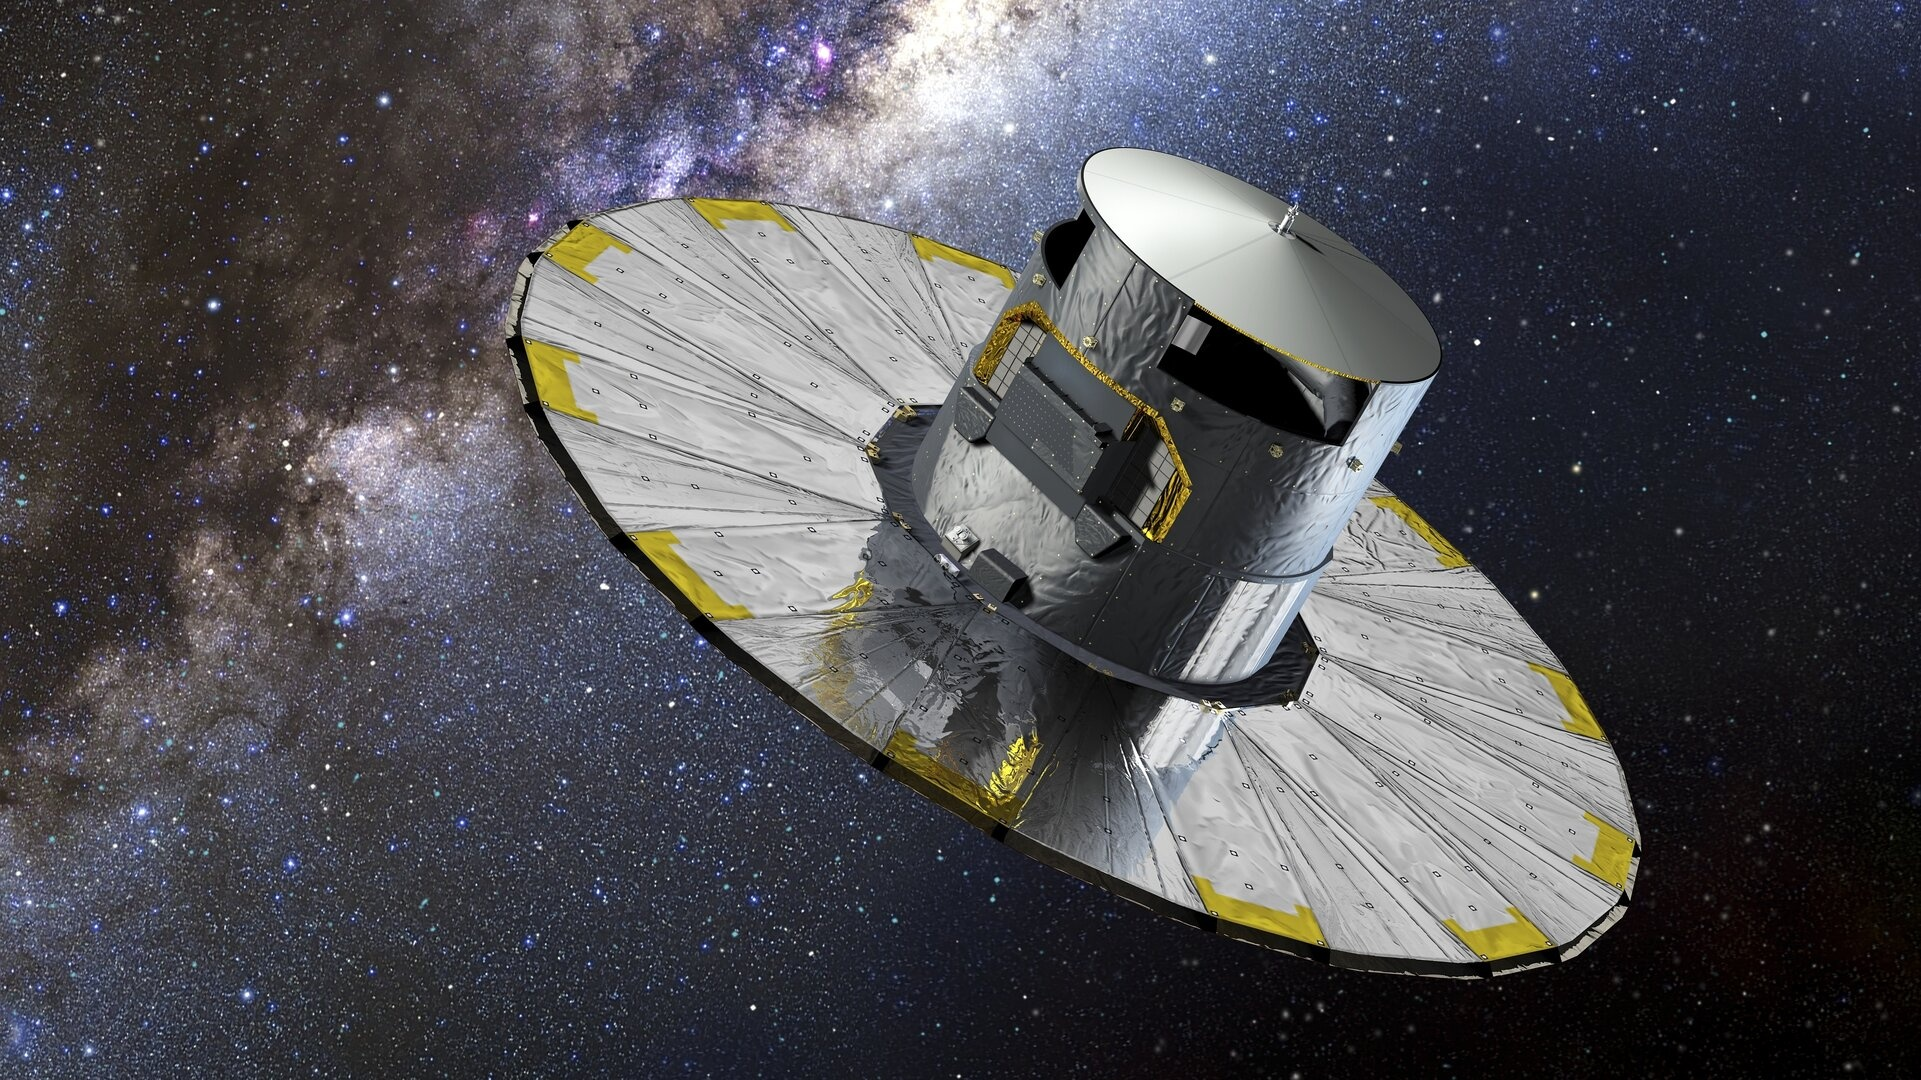
\includegraphics[width=\textwidth]{imaxes/gaia}
    \caption{Representación de la sonda Gaia}
    \label{fig:sonda}
\end{figure}

\subsection{Composición y estructura de los datos}\label{subsec:composicion}
El \textbf{Data Release 3 (DR3)}~\cite{gaia_dr3_documentation} de la misión Gaia constituye el conjunto de datos más completo y preciso publicado hasta la fecha por la ESA\@.
Fue presentado oficialmente el 13 de junio de 2022 e incluye observaciones recopiladas durante los primeros 34 meses de operación científica del satélite, entre julio de 2014 y mayo de 2017.
Este lanzamiento representa un avance sustancial respecto a los catálogos anteriores (DR1 y DR2), tanto en el número de estrellas registradas como en la calidad y variedad de los parámetros disponibles.

El catálogo contiene información astrométrica, fotométrica y espectroscópica de más de \textbf{1.800 millones de objetos}, de los cuales aproximadamente 1.500 millones poseen soluciones astrométricas completas, es decir, posición, paralaje(desplazamiento con respecto a las demás estrellas) y movimiento propio.
Esta información se almacena en distintas tablas temáticas.
A continuación se detallan las más relevantes y necesarias para este proyecto.
Cada fila de estas tablas representa un único objeto observado al que se asocia a un identificador numérico \texttt{source\_id} que permite identificarlo y cruzarlo con distintas tablas y catálogos.
\subsubsection{Tabla \texttt{gaia\_source}}
La tabla \texttt{gaia\_source} contiene los parámetros fundamentales de cada objeto observado.
Esta tabla contiene más de cien columnas y constituye la base de las demás tablas, pero para la realización de este proyecto solo son necesarias 9 de sus columnas:
\begin{itemize}
    \item \texttt{source\_id}: Identificador común mencionado anteriormente.
    Está construido mediante el sistema de indexación jerárquico HEALPix\footnote{HEALPix. Disponible en: \url{https://healpix.sourceforge.io/}{HEALPix - Features}}, lo que permite conocer la localización aproximada de la estrella en el cielo.
    Este identificador es único para cada fuente y se utiliza para realizar referencias cruzadas entre las distintas tablas del archivo Gaia y otras bases de datos astronómicas.

    \item \texttt{ra}($\alpha$): Ascensión Recta , expresada en grados y referida al sistema de coordenadas ecuatoriales (epoch J2016.0).
    \footnote{El término \textit{epoch 2016} indica la fecha de referencia para las coordenadas y los movimientos propios utilizados en el catálogo. En astronomía, las posiciones de las estrellas cambian lentamente con el tiempo debido a su movimiento real en el espacio y a efectos como la precesión. Por ello, los catálogos fijan una \textit{época} (en este caso el año 2016) como punto de referencia a partir del cual se definen y extrapolan las posiciones estelares.}
    Indica la posición de la fuente en el eje Este–Oeste del cielo y, junto con la declinación, determina su ubicación precisa en la bóveda celeste.

    \item \texttt{dec}($\delta$): Declinación , también en grados, medida en el sistema ecuatorial.
    Representa la posición angular de la fuente respecto al ecuador celeste, análoga a la latitud terrestre.
    Combinada con \texttt{ra}, define la posición bidimensional de la fuente observada.

    \item \texttt{pmra}: Movimiento propio en dirección de ascensión recta ($\mu_{\alpha}\cos\delta$), expresado en milisegundos de arco por año (mas/yr).
    Incluye el factor $\cos(\delta)$ para corregir la convergencia de meridianos hacia los polos.
    Indica el desplazamiento aparente de la fuente a lo largo del eje de ascensión recta debido a su movimiento real dentro de la galaxia.

    \item \texttt{pmdec}: Movimiento propio en dirección de declinación ($\mu_{\delta}$), también en mas/yr.
    Describe el desplazamiento aparente de la estrella en el eje Norte–Sur del cielo.
    Combinando \texttt{pmra} y \texttt{pmdec} puede calcularse la velocidad tangencial proyectada de la fuente, información esencial para el estudio cinemático de la Vía Láctea.

    \item \texttt{radial\_velocity}: Velocidad radial de la estrella respecto al Sol, expresada en km/s.
    Este parámetro se obtiene a partir del \textit{Radial Velocity Spectrometer} (RVS) a bordo de Gaia.
    Permite conocer el componente de la velocidad en la línea de visión y, junto con los movimientos propios, reconstruir el vector de movimiento tridimensional de la fuente.

    \item \texttt{phot\_g\_mean\_mag}: Magnitud aparente media en la banda fotométrica \texttt{G}, calibrada en el sistema Vega, es una medida directa del brillo observado.
    Este valor, combinado con la distancia, permite calcular la magnitud absoluta y, por tanto, la luminosidad estelar.

    \item \texttt{bp\_rp}: Color fotométrico definido como la diferencia entre las magnitudes medias en las bandas azul (\texttt{BP}) y roja (\texttt{RP}).
    Este índice de color es un indicador directo de la temperatura efectiva de la estrella.

    \item \texttt{logg\_gspphot}: Logaritmo de la gravedad superficial de la estrella, expresado en cm/s$^2$ y estimado por el módulo fotométrico \texttt{GSP-Phot}.
    Valores altos corresponden a estrellas de la secuencia principal, mientras que valores bajos son típicos de gigantes o supergigantes.
\end{itemize}
\subsubsection{Tabla \texttt{astrophysical\_parameters}}
Las columnas extraídas de la tabla \texttt{astrophysical\_parameters} pertenecen al módulo \texttt{FLAME} (\textit{Final Luminosity, Age and Mass Estimator}), encargado de estimar parámetros físicos de las estrellas a partir de la información fotométrica y de modelos de evolución estelar.
A continuación se describen las columnas empleadas en este trabajo:

\begin{itemize}
    \item \texttt{source\_id}: Identificador único de la fuente, común con la tabla \texttt{gaia\_source}.
    Es la clave primaria utilizada en las consultas cruzadas entre tablas.

    \item \texttt{mass\_flame}: Masa estelar estimada en unidades de masa solar ($M_{\odot}$). Este valor se obtiene mediante el ajuste de modelos teóricos de evolución estelar a las observaciones fotométricas y astrométricas (paralaje, temperatura efectiva, luminosidad y metalicidad).

    \item \texttt{radius\_flame}: Radio estelar estimado en unidades de radio solar ($R_{\odot}$), derivado de los mismos modelos empleados por el módulo \texttt{FLAME}.
    Este parámetro indica el tamaño físico aproximado de la estrella.
    En combinación con la temperatura efectiva y la luminosidad, permite situar la estrella dentro del diagrama de Hertzsprung–Russell\footnote{Más información disponible en: \url{https://es.wikipedia.org/wiki/Diagrama_de_Hertzsprung-Russell}} y estimar su estado evolutivo (secuencia principal, subgigante o gigante).
\end{itemize}
\subsubsection{Parámetro adicional}
Además de las columnas anteriores, se incluye también el parámetro \texttt{rgeo}, obtenido a través del servicio \textit{TAP VizieR}\footnote{TAP VizieR. Disponible en: \url{https://tapvizier.u-strasbg.fr/adql/}}, que proporciona datos complementarios derivados de catálogos externos al archivo principal de Gaia:

\begin{itemize}
    \item \texttt{rgeo}: Distancia geométrica estimada en parsecs (pc)\footnote{1 pc equivale a 3.26 años luz o 3,0857 \times 10^{13}km} basada en el método bayesiano desarrollado por Bailer-Jones~\cite{Bailer-Jones2021}.
    Este parámetro corrige las incertidumbres y sesgos asociados al cálculo directo de la distancia mediante la inversa del paralaje, especialmente relevantes en regiones con errores elevados o valores negativos de paralaje.
    El valor de \texttt{rgeo} representa la mejor estimación estadística de la distancia a la fuente, teniendo en cuenta tanto la medida observacional como un modelo de distribución espacial de estrellas en la galaxia.
    Resulta fundamental para convertir magnitudes aparentes en magnitudes absolutas y para estimar luminosidades físicas de las estrellas con mayor precisión.
\end{itemize}

\section{Selección y filtrado de los datos}\label{sec:filtrado}
El catálogo \textbf{Gaia DR3} contiene información astrométrica, fotométrica y espectroscópica de más de \textbf{1.800 millones de fuentes}.
Sin embargo, para los objetivos de este trabajo no todas las fuentes son adecuadas, ya que poblaciones evolucionadas (gigantes, subgigantes o enanas blancas) presentan cinemáticas y distribuciones espaciales distintas, lo que impide calcular adecuadamente algunos de sus parámetros.

Por esta razón, se selecciona únicamente la población de \textbf{estrellas de la secuencia principal}, definida en el diagrama color–magnitud por el intervalo fotométrico:

\[
    0.3 < (BP - RP) < 2.0.
\]

Esta restricción garantiza que las estrellas analizadas se encuentren en una fase estable de evolución estelar, dominada por la fusión de hidrógeno en el núcleo.

Adicionalmente, se descartan todas las fuentes con información incompleta, es decir, aquellas que presentan valores nulos (\texttt{NULL}) en alguna de las siguientes columnas esenciales:
\texttt{bp\_rp}, \texttt{phot\_g\_mean\_mag} o \texttt{rgeo}.
Este filtrado no solo garantiza la coherencia de las magnitudes físicas calculadas, sino que también reduce el tamaño efectivo del conjunto de datos, lo cual es crucial desde el punto de vista computacional.

Tras aplicar ambos criterios, la restricción fotométrica de secuencia principal y la eliminación de registros incompletos, la muestra final empleada en este trabajo queda compuesta por \textbf{1.174.075.109 estrellas}.

\section{Transformación de los datos}\label{sec:calculos_previos}

Para poder computar la dispersión estelar necesitamos caracterizar completamente la posición, el movimiento y las propiedades fundamentales de cada estrella utilizando un sistema de referencia coherente.
En esta sección describimos cómo transformamos los datos disponibles en el catálogo Gaia DR3 para obtener las magnitudes físicas  y espaciales que vamos a necesitar.
\subsection{Transformación de coordenadas}\label{subsec:transformacion-de-coordenadas}

Las coordenadas ecuatoriales $(\alpha, \delta)$ describen la posición de una estrella en la esfera celeste tomando como referencia el ecuador terrestre proyectado en el cielo.
No obstante, para estudiar la estructura y dinámica de la Vía Láctea resulta más útil emplear un sistema de referencia ligado a su propio plano.
Este sistema es el de \textbf{coordenadas galácticas}, en el cual las posiciones se expresan respecto al centro de la galaxia.

En este sistema:
\begin{itemize}
    \item El \textbf{origen} se sitúa en el \textbf{centro galáctico}.
    \item El eje $X$ apunta hacia el \textbf{centro galáctico} (dirección de la constelación de Sagitario).
    \item El eje $Z$ apunta hacia el \textbf{polo norte galáctico}, perpendicular al plano galáctico.
    \item El eje $Y$ completa el sistema formando una base dextrógira (regla de la mano derecha).
\end{itemize}

La conversión entre coordenadas ecuatoriales y galácticas puede expresarse como una rotación en el espacio tridimensional.
La orientación del plano galáctico fue definida por la IAU, y la matriz de rotación asociada es:

\[
    \mathbf{R} =
    \begin{bmatrix}
        -0.05487556 & -0.87343709 & -0.48383502 \\
        +0.49410943 & -0.44482963 & +0.74698225 \\
        -0.86766615 & -0.19807637 & +0.45598380
    \end{bmatrix},
\]

cuyas constantes fueron establecidas por Murray (1989) y continúan siendo el estándar actual en herramientas astrométricas modernas como \texttt{Astropy}~\cite{murray1989_coordinates}.
Dado que el sistema de referencia de Gaia DR3 está alineado con el ICRS (Sistema de Referencia Celeste Internacional), esta matriz es directamente aplicable a los datos utilizados en este trabajo.

Para una estrella situada a una distancia heliocéntrica $d$ (en parsecs), se construye primero el vector de posición unitario en el sistema ecuatorial:

\[
    \hat{\mathbf{r}}_E =
    \begin{pmatrix}
        \cos \delta \cos \alpha \\
        \cos \delta \sin \alpha \\
        \sin \delta
    \end{pmatrix}
\]

Al multiplicarlo por la matriz $\mathbf{R}$ obtenemos la dirección en el sistema galáctico, y al escalar por $d/1000$ expresamos la posición en kiloparsecs:

\[
    \begin{pmatrix}
        X \\ Y \\ Z
    \end{pmatrix}
    =
    \frac{d}{1000}\,
    \mathbf{R}\,
    \hat{\mathbf{r}}_E
\]

Esta transformación permite situar la estrella en un sistema de referencia coherente con la geometría de la Vía Láctea, lo cual es fundamental para el análisis de su estructura y distribución espacial.

\subsection{Estimación de la Velocidad Radial}\label{subsec:estimacion-de-la-velocidad-radial}
La velocidad radial \( v_r \) representa la componente de la velocidad estelar proyectada a lo largo de la línea de visión del observador.
En caso de no estar disponible en el catálogo para una determinada estrella, se realiza una estimación basada en su posición y movimientos propios, aplicando la formulación clásica de Johnson \& Soderblom~\cite{johnson1987}.


El punto de partida son los movimientos propios en ascensión recta y declinación (\( \mu_{\alpha} \)) y (\( \mu_{\delta} \)), los cuales describen cómo cambia la posición aparente de la estrella en la esfera celeste.
Estos movimientos propios corresponden únicamente a la componente tangencial de la velocidad estelar, es decir, perpendicular a la línea de visión.
Para convertirlos en una velocidad física en el espacio, es necesario combinarlos con la distancia \( d \) a la estrella.

Primero, calculamos la velocidad tangencial tridimensional.
Para ello se utiliza una matriz de transformación \( T \) , que permite transformar las variaciones angulares observadas sobre la esfera celeste en componentes cartesianas en un sistema de coordenadas ecuatoriales:
\[
    T =
    \begin{pmatrix}
        -\sin\alpha & -\cos\alpha \sin\delta \\
        \cos\alpha & -\sin\alpha \sin\delta \\
        0 & \cos\delta
    \end{pmatrix}
\]

donde \(\alpha\) y \(\delta\) son la ascensión recta y la declinación de la estrella.
La velocidad tangencial resultante se obtiene como:

\[
    \vec{V} = \kappa \, d \,
    T
    \begin{pmatrix}
        \mu_{\alpha} \\
        \mu_{\delta}
    \end{pmatrix}
\]

donde \(\kappa = 4.74047\) es el factor de conversión entre movimiento propio (en mas/año), distancia (en parsecs) y velocidad (en km/s).

Posteriormente, la proyección de este vector sobre la dirección de la línea de visión (definida por las coordenadas galactocéntricas \( C_x, C_y, C_z \)) proporciona una primera estimación de la componente radial.
\[
    V_{\text{radial\_sin}} =
    \frac{C_x V_x + C_y V_y + C_z V_z}
    {\sqrt{C_x^2 + C_y^2 + C_z^2}}
\]
A esta estimación se le añaden dos correcciones:

\begin{enumerate}
    \item \textbf{Corrección por rotación galáctica}, calculada como:
    \[
        V_{\text{rot}} = V_{\text{GAL}} \frac{C_y}{\sqrt{C_x^2 + C_y^2}}
    \]
    donde \( V_{\text{GAL}} \) es la velocidad de rotación del Sol alrededor del centro galáctico.

    \item \textbf{Corrección por el movimiento peculiar del Sol}, determinada mediante:
    \[
        V_{\text{sol}} = \frac{U_{\text{SOL}} C_x + V_{\text{SOL}} C_y + W_{\text{SOL}} C_z}{\sqrt{C_x^2 + C_y^2 + C_z^2}}
    \]
    donde \( (U_{\text{SOL}}, V_{\text{SOL}}, W_{\text{SOL}}) \) representan las componentes de la velocidad solar respecto al entorno local.
\end{enumerate}

Finalmente, la velocidad radial estimada se obtiene como:

\[
    v_r = V_{\text{radial\_sin}} + V_{\text{rot}} - V_{\text{sol}}
\]
En este trabajo se adoptan los valores propuestos por Schönrich et al\cite{schonrich2010,blandhawthorn2016} para el movimiento solar:
\( V_{\text{GAL}} = 220~\text{km s}^{-1} \), \( U_{\text{SOL}} = 11.1~\text{km s}^{-1}\), \( V_{\text{SOL}} = 12.24~\text{km s}^{-1}\), \( W_{\text{SOL}} = 7.25~\text{km s}^{-1}\).

De este modo, el procedimiento permite aproximar la velocidad radial de una estrella a partir de parámetros astrométricos disponibles (posición, movimientos propios y distancia), incluyendo los efectos de la rotación galáctica y del movimiento solar.
\subsection{Cálculo de las velocidades espaciales}\label{subsec:calculo-de-las-velocidades-espaciales}

A través de los movimientos propios observados en ascensión recta y declinación, \(\mu_{\alpha}\cos\delta\) y \(\mu_{\delta}\) (expresados en mas\,año\(^{-1}\)), junto con una distancia \(d\) (en parsec) y una velocidad radial observada \(V_r\) (en km\,s\(^{-1}\)), es posible determinar las componentes de la velocidad espacial en el sistema galáctico \((V_X, V_Y, V_Z)\).

El cálculo se basa en la conversión de las magnitudes observadas (coordenadas ecuatoriales) al sistema cartesiano galáctico utilizando de nuevo la formulación de Johnson \& Soderblom~\cite{johnson1987}.
Primero se obtiene la velocidad tangencial en las direcciones de ascensión recta y declinación mediante:
\[
    V_{t,\alpha} = \kappa \, d \, \mu_{\alpha}\cos\delta,
    \qquad
    V_{t,\delta} = \kappa \, d \, \mu_{\delta},
\]

donde \(\kappa = 4.74047\) es el factor de conversión que relaciona movimientos propios (mas\,año\(^{-1}\)) y distancias (pc) con velocidades en km\,s\(^{-1}\).

A partir de la velocidad radial \(V_r\) y de las velocidades tangenciales \(V_{t,\alpha}\) y \(V_{t,\delta}\),
se calcula el vector velocidad en el sistema ecuatorial:

\[
    \vec{V}_E' = V_r\,\hat{\mathbf{r}}_E + T
    \begin{pmatrix}
        V_{t,\alpha} \\
        V_{t,\delta}
    \end{pmatrix}
\]

donde \(\hat{\mathbf{r}}_E\) es el vector unitario que apunta hacia la estrella en coordenadas ecuatoriales,
y \(T\) es la matriz que proyecta las velocidades tangenciales sobre el sistema cartesiano ecuatorial definidas con anterioridad.

Finalmente, para obtener las componentes de velocidad en el sistema de referencia galáctico,
se aplica una rotación mediante la matriz \(R\) vista anteriormente, que transforma las coordenadas ecuatoriales al sistema galáctico:

\[
    \begin{pmatrix}
        V_X \\
        V_Y \\
        V_Z
    \end{pmatrix}
    =
    R \cdot
    \vec{V}_E'
    \cdot \Sigma,
\]

donde \(\Sigma = 0.0010227\) es el factor de conversión de km\,s\(^{-1}\) a kiloparsec por millón de años (kpc\,Myr\(^{-1}\)).

De este modo, se obtienen las componentes \((V_X, V_Y, V_Z)\) en el sistema galáctico,
que describen el movimiento tridimensional de la estrella respecto al centro galáctico,
expresadas en unidades de kiloparsecs por millón de años (kpc\,Myr\(^{-1}\)).
\subsection{Estimación de masas estelares}\label{subsec:estimacion-de-masas-estelares}

Para las estrellas con parámetros atmosféricos conocidos, la masa se estima a partir de la relación entre la gravedad superficial $g$ y el radio estelar $R$~\cite{carroll2017}:

\[
    \log_{10}\left(\frac{M}{M_\odot}\right) = \log g - \log g_\odot + 2 \log_{10}\left(\frac{R}{R_\odot}\right)
\]

donde $\log g_\odot = 4.437$ es el valor adoptado para el Sol.
En los casos en los que la estimación directa no es posible, se aplica una relación empírica entre la masa, el color fotométrico $(BP-RP)$ y la magnitud absoluta $M_G$, siguiendo la metodología del módulo FLAME de Gaia DR3~\cite{gaia_dr3_flame}:

\[
    \log_{10}\left(\frac{M}{M_\odot}\right) = a \,(BP-RP) + b \, M_G + c
\]

con coeficientes ajustados para estrellas de la secuencia principal solar–metalicidad:
$a = -0.15$, $b = -0.10$, $c = 1.2$.
Esta aproximación permite mantener la coherencia de los datos incluso para fuentes incompletas, proporcionando una estimación razonable de la masa estelar en ausencia de mediciones directas.
\bigskip

Tras estos cálculos previos y las correspondientes transformaciones, se obtienen los datos necesarios en las unidades adecuadas para realizar los cálculos de dispersión estelar:

\begin{itemize}
    \item \textbf{Posición galactocéntrica} en kiloparsecs: \((C_X, C_Y, C_Z)\)
    \item \textbf{Velocidad galactocéntrica} en kiloparsecs por millón de años: \((V_X, V_Y, V_Z)\)
    \item \textbf{Masa estelar} en masas solares: \textit{mass}
\end{itemize}

\section{Cálculo de la dispersión estelar}\label{sec:dispersion}

Tras obtener las posiciones y velocidades galactocéntricas de las estrellas, el objetivo de esta sección es describir de forma detallada el marco físico y matemático empleado para calcular la dispersión estelar del sistema.
Se presentan los modelos del potencial galáctico, la forma en que se calculan las aceleraciones que rigen la dinámica del sistema y el integrador utilizado para la simulación.

\subsection{Esquema de integración temporal}\label{subsec:esquema-de-integracion-temporal-(leapfrog-kick--drift--kick).}
Para la realizar la simulación propiamente se emplea un integrador simétrico de segundo orden tipo \emph{Leapfrog} conocido como Kick--Drift--Kick~\cite{hockney1988,saha1992,springel2005}.
Este integrador realiza actualizaciones de velocidad (v) a mitad de paso y de posicion (r) a paso completo.
Denotando por \(\Delta t\) el paso temporal, las actualizaciones discretas son:
\[
    \begin{aligned}
        \mathbf{v}\!\left(t+\tfrac{\Delta t}{2}\right) &= \mathbf{v}(t) + \tfrac{\Delta t}{2}\,\mathbf{a}(t), \\[6pt]
        \mathbf{r}(t+\Delta t) &= \mathbf{r}(t) + \Delta t \,\mathbf{v}\!\left(t+\tfrac{\Delta t}{2}\right), \\[6pt]
        \mathbf{v}(t+\Delta t) &= \mathbf{v}\!\left(t+\tfrac{\Delta t}{2}\right) + \tfrac{\Delta t}{2}\,\mathbf{a}(t+\Delta t).
    \end{aligned}
\]
Este esquema es \(\mathcal{O}(\Delta t^2)\) en precisión y conserva bien las cantidades integrales (energía, momento angular) sobre escalas temporales largas, siendo por ello conveniente para simulaciones N-body de estructuras galácticas.


Para garantizar la estabilidad numérica y evitar que una estrella se desplace una distancia significativa en un solo paso de integración, el valor del paso temporal se fija de acuerdo con la velocidad máxima del sistema~\cite{dehnen2011,hockney1988}.
Sea \(v_{\max}\) la mayor velocidad galactocéntrica entre todas las estrellas y \(l_{\min}\) la escala espacial mínima resoluble.
El paso temporal máximo adoptado se calcula como
\[
    \Delta t_{\max} \;=\; \eta \, \frac{l_{\min}}{v_{\max}},
\]
donde \(\eta < 1\) es un factor de seguridad que limita el desplazamiento de cada partícula a una fracción de la resolución espacial en cada iteración.

De este modo, ninguna estrella puede recorrer una distancia superior a \(\eta\,l_{\min}\) en un único paso, lo que asegura que las aceleraciones se actualicen con suficiente frecuencia y que la integración \emph{Leapfrog Kick–Drift–Kick} conserve la energía y momento angular del sistema de forma estable.

\subsection{Aceleraciones en el sistema}\label{subsec:aceleraciones-en-el-sistema}
En cada paso del integrador, es necesario evaluar la aceleración total \(\mathbf{a}_i\) que actúa sobre cada estrella \(i\).
Esta aceleración se descompone en dos componentes principales:
\[
    \mathbf{a}_i = \mathbf{a}_{\mathrm{gal}}(\mathbf{r}_i) + \mathbf{a}_{\star-\star,i},
\]
donde \(\mathbf{a}_{\mathrm{gal}}\) es la aceleración analítica producida por el potencial galáctico fijo (halo + bulbo), y \(\mathbf{a}_{\star-\star,i}\) representa la contribución debida a las interacciones gravitatorias con las demás estrellas simuladas, lo que corresponde con el mayor coste computacional de la simulación.
\subsubsection{Aceleraciones analíticas}
\begin{itemize}
    \item \textbf{Aceleración del halo} (\(\mathbf{a}_{\mathrm{halo}}\)): representa la contribución del \emph{halo de materia oscura}, el cual domina la masa en la región externa de la galaxia.
    Se modela con un perfil NFW (Navarro–Frenk–White)~\cite{navarro1996}, cuya simetría esférica permite expresar su aceleración como función únicamente del radio galactocéntrico \(r\).
    \[
        \mathbf{a}_{\mathrm{halo}}(\mathbf{r}) = -\,\frac{G\,M_{\mathrm{enc}}(r)}{r^3}\,\mathbf{r}.
    \]
    Este término impone el campo gravitacional de gran escala, responsable de mantener la rotación galáctica aproximadamente plana.

    \item \textbf{Aceleración del bulbo} (\(\mathbf{a}_{\mathrm{bulge}}\)): describe la atracción generada por la masa concentrada en el centro galáctico.
    Se adopta el potencial de Hernquist, que reproduce la distribución de densidad de los bulbos~\cite{hernquist1990}:
    \[
        \mathbf{a}_{\mathrm{bulge}}(\mathbf{r}) = -\,\frac{G\,M_b}{r(r+a)^2}\,\mathbf{r}.
    \]
    Su efecto domina en las regiones centrales, proporcionando el confinamiento gravitatorio más intenso.
\end{itemize}
\subsubsection{Interacciones entre estrellas}
La contribución debida a las interacciones mutuas entre estrellas se obtiene a partir de la ley de gravitación de Newton.
Para dos partículas puntuales de masas \(m_i\) y \(m_j\) ubicadas en \(\mathbf{r}_i\) y \(\mathbf{r}_j\), la fuerza de atracción entre ellas será:
\[
    \mathbf{F}_{ij} \;=\; - G \, \frac{m_i m_j}{(|\mathbf{r}_i-\mathbf{r}_j|^2 + \varepsilon^2)^{3/2}} \, (\mathbf{r}_i - \mathbf{r}_j),
\]
donde \(\varepsilon\) es el parámetro de \emph{suavizado} (softening) introducido para evitar singularidades y efectos extraños en corta distancia~\cite{hockney1988}.
La aceleración sobre la partícula \(i\) por parte de \(j\) es entonces:
\[
    \mathbf{a}_{ij} \;=\; - G \, \frac{m_j}{(|\mathbf{r}_i-\mathbf{r}_j|^2 + \varepsilon^2)^{3/2}} \, (\mathbf{r}_i - \mathbf{r}_j).
\]
La aceleración de las interacciones sobre la estrella \(i\) es la suma de todas las contribuciones estelares:
\[
    \mathbf{a}_i \;=\; \sum_{j\neq i} \mathbf{a}_{ij}.
\]
Calcular exactamente la suma de las aceleraciones para todas las estrellas conduce a un coste \(O(N^2)\) lo que resulta inviable para un N grande.

Para reducir el coste computacional de la suma sobre \(j\), se puede aproximar la contribución de grupos de partículas lejanas por su masa total y centro de masa, lo que se conoce como aproximación multipolar o criterio de Barnes-Hut~\cite{barnes1986}.
Si un grupo de tamaño característico \(s\) está a distancia \(d\) del cuerpo considerado, el criterio de apertura \(\theta\) de Barnes--Hut decide si la celda puede tratarse como un único cuerpo:
\[
    \frac{s}{d} < \theta \quad \Longrightarrow \quad
    \mathbf{a}_{\text{celda}} \approx - G \, \frac{M_{\text{celda}}}{d^2} \,\hat{\mathbf{d}} .
\]
Si la desigualdad no se cumple, la celda se subdivide y se consideran sus hijos (multipolo de orden superior si se desea mayor precisión).
El parámetro \(\theta\) controla la precisión/velocidad.


 \chapter{Fundamentos tecnológicos}\label{ch:fundamentos}

\lettrine{E}{n} este capítulo se describen los recursos hardware y software empleados durante la realización del proyecto.
Se detalla la infraestructura física utilizada —el superordenador \textbf{Finisterrae III}— y las principales herramientas de software necesarias para la ejecución, análisis y optimización de los experimentos realizados.


\section{Infraestructura física: Finisterrae III}\label{sec:infraestructura-fisica}

Para la ejecución de las simulaciones y experimentos descritos en este trabajo se ha empleado una infraestructura de computación de altas prestaciones (\textit{High Performance Computing}, HPC).
En particular, se ha utilizado el supercomputador \textbf{Finisterrae III}, ubicado en el Centro de Supercomputación de Galicia (CESGA)\footnote{Información oficial disponible en \url{https://www.cesga.es/infraestructuras/computacion/}}.

El Finisterrae III constituye una plataforma HPC moderna, con una elevada capacidad de cómputo, memoria y almacenamiento.
Dispone de un total de 22.848 núcleos de CPU y 171 GPU, distribuidas en 357 nodos interconectados mediante una red \textit{InfiniBand HDR}.
Su potencia bruta asciende a \textbf{4,36 PetaFLOPS}.
\begin{figure}[hp!]
    \centering
    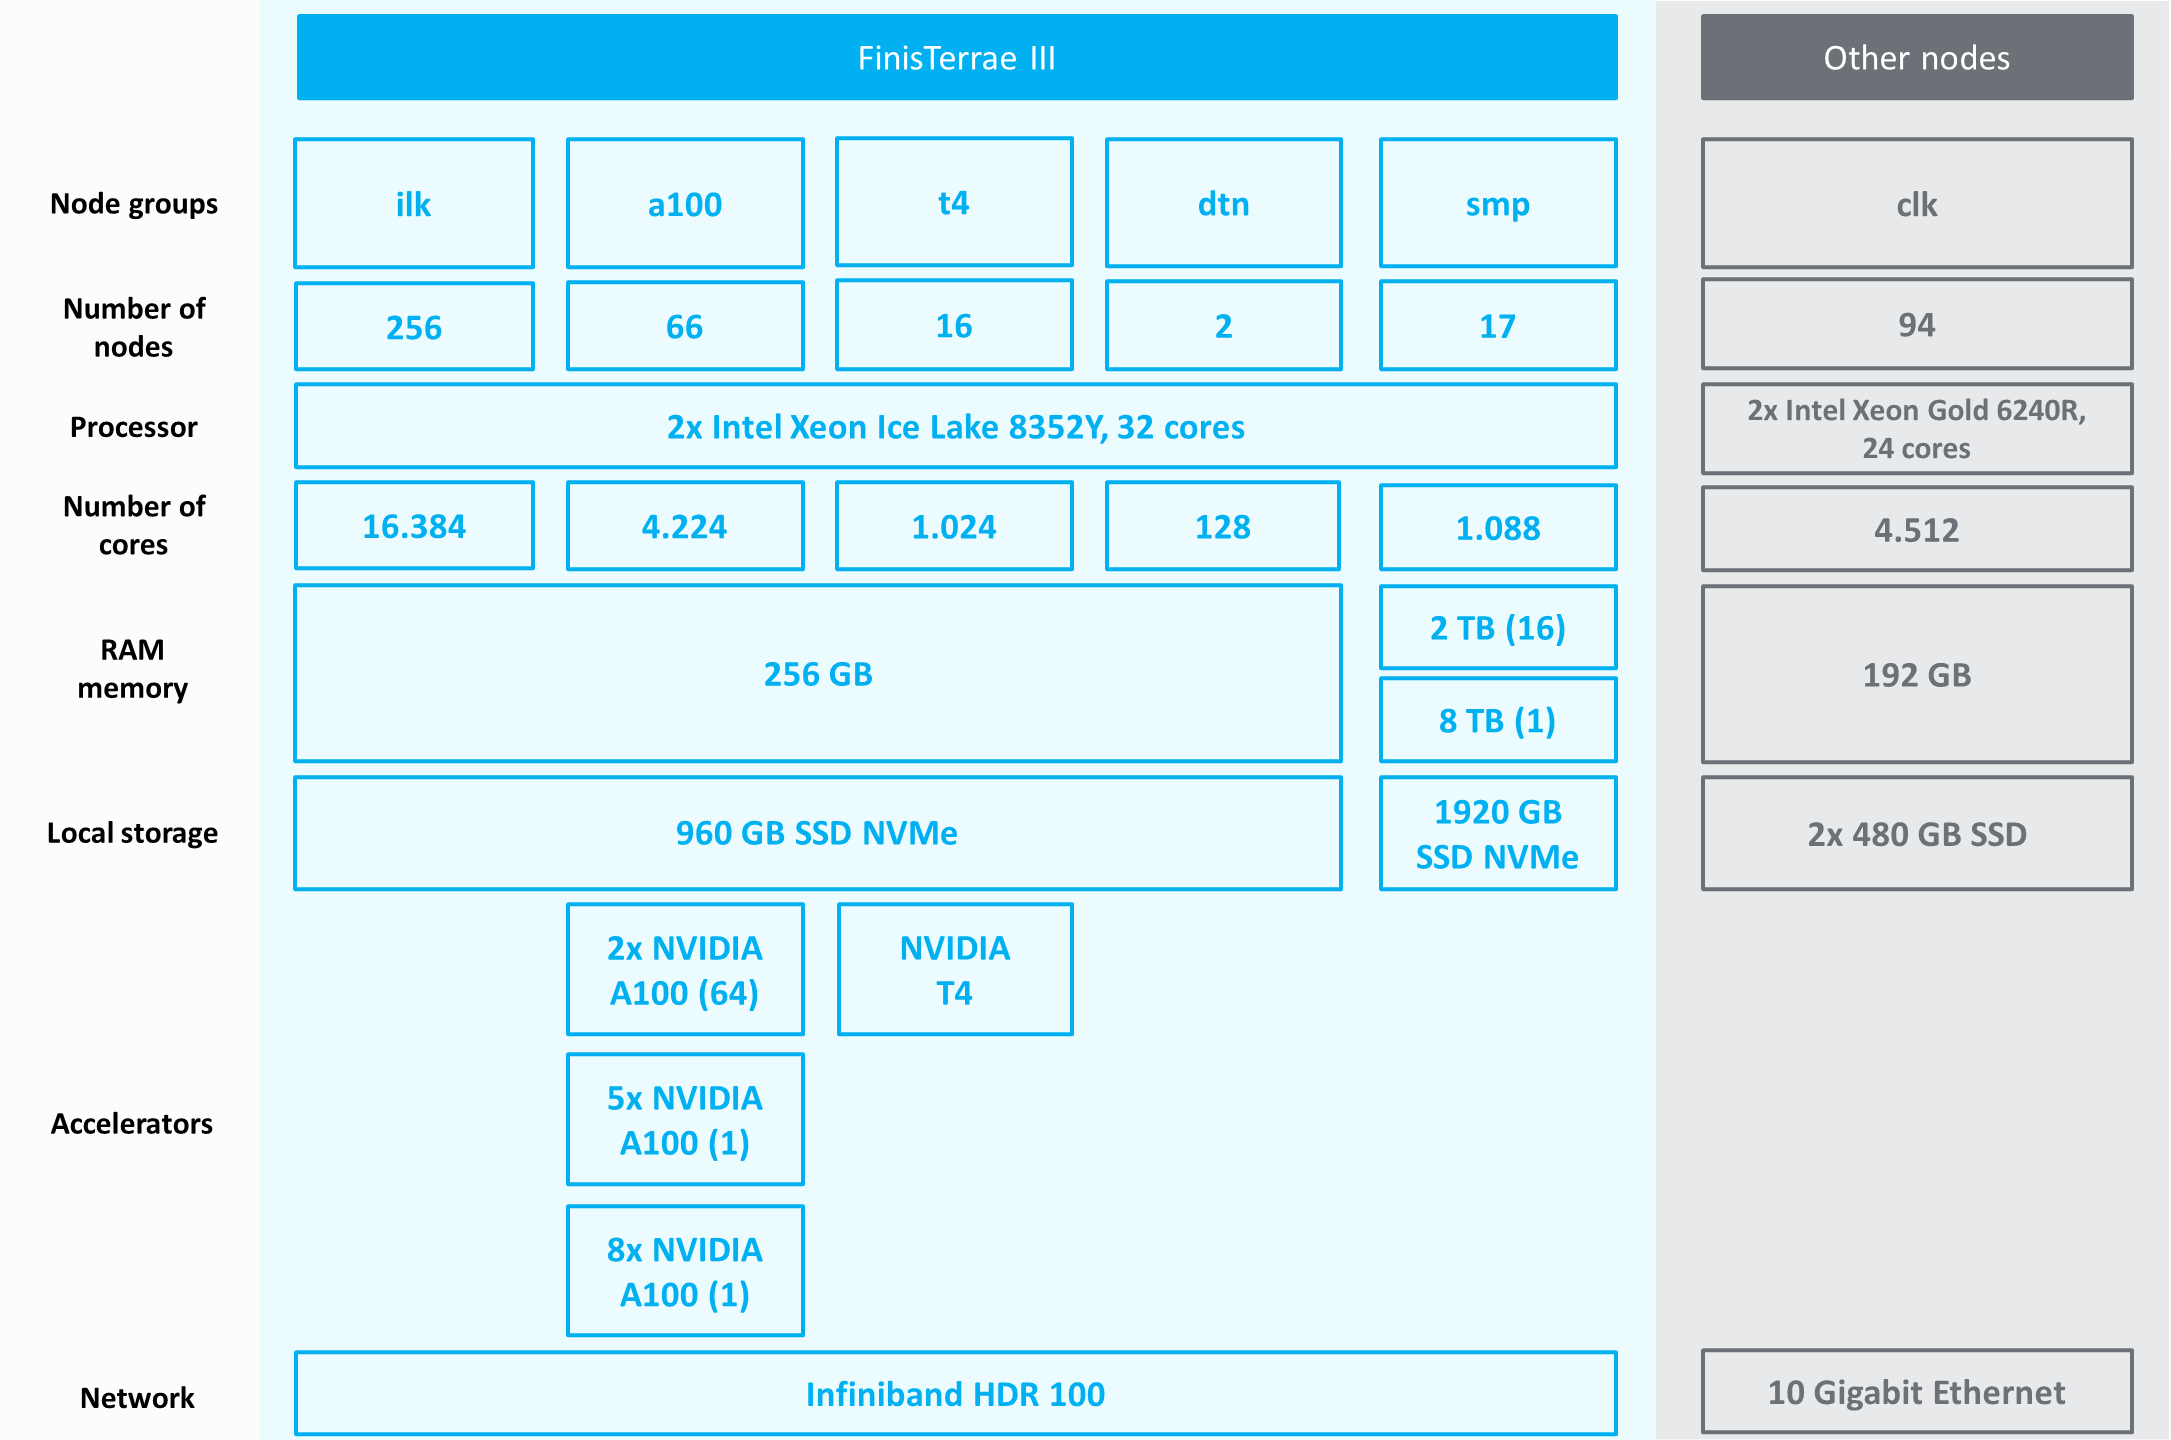
\includegraphics[width=\textwidth]{imaxes/FT3_schema}
    \caption{Esquema general de la arquitectura del supercomputador Finisterrae III}
    \label{fig:ft3-scheme}
\end{figure}

\subsection{Especificaciones técnicas de los nodos}\label{subsec:especificaciones-tecnicas-de-los-nodos}

La arquitectura del sistema se organiza en distintos tipos de nodos según el tipo de tarea a realizar tal y como se muestra en la figura~\ref{fig:ft3-scheme}.
Para este proyecto se han empleado cuatro clases de nodos:

\begin{itemize}
    \item \textbf{Nodos \texttt{ilk} (CPU)}: Diseñados para tareas de cómputo intensivo que no requieren aceleración por GPU. El Finisterrae III cuenta con 256 de estos nodos.
    Necesario para la versión cpu del proyecto.
    \item \textbf{Nodos \texttt{a100} (GPU)}: Equipados con unidades de procesamiento gráfico NVIDIA A100, orientados a cargas de trabajo en inteligencia artificial y procesamiento masivo de datos.
    Existen 64 nodos de este tipo.
    Necesario para simulaciones con hasta 2 GPUs.
    \item \textbf{Nodos \texttt{smp} (MEM)}: Similares a los nodos \texttt{ilk}, pero con una capacidad de memoria superior (2~TB), adecuados para trabajos que requieren un elevado uso de memoria.
    Necesario para la realización de pruebas de tamaño del árbol, tamaño de la base de datos y de resultados.
    \item \textbf{Nodo \texttt{a100-m8}}: Nodo especial para entrenamiento de modelos de IA y procesamiento multi-GPU, que dispone de 8 GPU NVIDIA A100 y mayor capacidad de memoria RAM.
    Necesario para la realización de simulaciones con más de 2 GPUs.
\end{itemize}

\subsection{Sistema de almacenamiento}\label{subsec:sistema-de-almacenamiento}

Además de los nodos de cómputo, el sistema cuenta con un almacenamiento en red de alta capacidad accesible desde todos los nodos.
Este almacenamiento está dividido en distintas áreas con cuotas y políticas específicas:

\begin{itemize}
    \item \textbf{\$HOME}: Espacio destinado a código fuente y programas. 
    Conectado mediante un enlace de baja velocidad, con límite de 10~GB o 100.000 archivos. 
    Incluye copias de seguridad diarias durante dos meses y \textit{snapshots} semanales.
    En el proyecto se utiliza para almacenar el código fuente, scripts y resultados de tests.
    \item \textbf{\$STORE}: Orientado al almacenamiento de resultados finales. 
    Límite de 500~GB o 300.000 archivos.
    Posee \textit{snapshots} durante tres días, sin copia de seguridad.
    Debido al poco espacio que ofrece, no es posible almacenar los resultados del proyecto en esta partición, por lo que no se utiliza.
    \item \textbf{\$LUSTRE}: Sistema de archivos de alta velocidad, destinado a la ejecución de simulaciones.
    No dispone de copias de seguridad ni \textit{snapshots}, y está limitado a 3~TB o 200.000 archivos.
    Gracias a su alta velocidad y la posibilidad de leer y escribir paralelamente archivos con gran eficiencia, se destina a almacenar y transformar los datos iniciales, así como almacenar los resultados finales.
\end{itemize}

\subsection{Modos de acceso}\label{subsec:modos-de-acceso}

El sistema ofrece cuatro modalidades principales de uso, en función del nivel de interactividad y la carga computacional requerida:

\begin{enumerate}
    \item \textbf{Uso interactivo}: acceso limitado y compartido mediante los nodos de \textit{login} (máximo 8~GB de memoria virtual).
    \item \textbf{Escritorios remotos}: acceso gráfico completo mediante X11; permite ejecutar aplicaciones con interfaz gráfica, aunque no es recomendable para simulaciones largas o que superen los 32~GB de memoria.
    \item \textbf{Nodos interactivos dedicados}: sesiones interactivas con recursos exclusivos mediante el comando \texttt{compute}, con un máximo de 64 núcleos y 247~GB de RAM durante 8 horas.
    \item \textbf{Sistema de colas}: uso mediante el gestor de colas \textbf{Slurm Workload Manager}~\cite{slurm}, indicado para simulaciones prolongadas o de gran escala.
    Los trabajos se envían mediante el comando \texttt{sbatch} (modo no interactivo) o \texttt{srun} (modo interactivo).
\end{enumerate}

En este proyecto se ha utilizado principalmente el sistema de colas de \textbf{Slurm} para las simulaciones, combinándolo con escritorios remotos para la ejecución de herramientas gráficas de análisis.
El acceso al sistema se realiza mediante SSH (\textit{Secure Shell}), utilizando el comando ssh user\_cesga@ft3.cesga.es.
El usuario es redirigido automáticamente a uno de los nodos de \textit{login}, desde los cuales se puede compilar software, preparar scripts o enviar trabajos al planificador.

\subsection{Módulos software}\label{subsec:modulos-software}
La gestión de aplicaciones en Finisterrae III se realiza mediante el sistema de módulos \textbf{Lmod}\footnote{Lmod: Environment Modules System. Disponible en: \url{https://lmod.readthedocs.io/}}, que permite cargar entornos modulares y establecer las variables de entorno correspondientes.
Dado el elevado número de dependencias entre aplicaciones y versiones, es necesario cargar un módulo jerárquico principal.
En este proyecto se ha utilizado el entorno base \texttt{cesga/2025}.

Los principales módulos empleados fueron:

\begin{itemize}
    \item \textbf{CMake}\footnote{CMake. Disponible en:\url{https://cmake.org/}}:
    Es una herramienta de automatización del proceso de compilación que permite generar de manera portable los archivos necesarios para construir proyectos en distintos sistemas y compiladores.
    En este caso facilita la gestión de dependencias, la compilación modular y la consistencia de pruebas locales y en la infraestructura HPC\@.

    \item \textbf{OpenMP}:
    Es una API que permite la programación paralela en sistemas de memoria compartida.
    Para una descripción detallada, véase la sección~\ref{subsec:openmp}.
    \item \textbf{CUDA}:
    Es una plataforma de computación paralela y un modelo de programación desarrollado por NVIDIA diseñado para aprovechar la potencia de sus GPUs con todo tipo de cálculos.
    Para una descripción detallada, véase la sección~\ref{subsec:cuda}.

    \item \textbf{Intel Compiler}:
    Es un conjunto de compiladores diseñados para obtener el máximo rendimiento en procesadores fabricados por Intel.
    Proporciona optimizaciones automáticas a nivel de vectorización, paralelización y uso eficiente de la memoria caché.

    \item \textbf{Intel VTune Profiler}\footnote{Intel VTune Profiler. Disponible en:\url{https://www.intel.com/content/www/us/en/developer/tools/vtune-profiler.html}}:
    Es una herramienta de análisis y perfilado de rendimiento desarrollada por Intel.
    Permite detectar cuellos de botella en el uso de CPU, memoria o E/S, ofreciendo métricas detalladas sobre la ejecución de los programas.
    Su integración con los compiladores Intel facilita la optimización iterativa del código y la evaluación del impacto de las mejoras implementadas.

    \item \textbf{NVIDIA HPC Compiler}:
    Forma parte del conjunto \textit{NVIDIA HPC SDK}, que incluye compiladores, bibliotecas y herramientas optimizadas para el desarrollo de aplicaciones de alto rendimiento en CPU y GPU.
    Especialmente diseñado para la compilación de aplicaciones CUDA de alto rendimiento.
    Además, proporcionan optimizaciones automáticas para GPU NVIDIA A100, como las presentes en el supercomputador Finisterrae III.

    \item \textbf{NVIDIA Nsight Compute}\footnote{Nvidia Nsight Compute. Disponible en:\url{https://developer.nvidia.com/nsight-compute}}:
    Es un analizador de rendimiento (\textit{profiler}) especializado para aplicaciones CUDA.
    Permite inspeccionar la ejecución de kernels en GPU, analizando métricas como la utilización de memoria global, el rendimiento de cada multiprocesador o el grado de ocupación de los núcleos CUDA.
    Es una herramienta fundamental para optimizar aplicaciones paralelas que utilizan GPU NVIDIA.

\end{itemize}

\section{Tecnologías de paralelización: OpenMP y CUDA}\label{sec:openmp-cuda}
En este proyecto se han empleado dos tecnologías principales para la paralelización del código: OpenMP, orientada a sistemas de memoria compartida, y CUDA, diseñada para aprovechar la capacidad de cómputo masivo de las GPU NVIDIA\@.

\subsection{OpenMP}\label{subsec:openmp}

\textbf{OpenMP}~\cite{openmp-spec} es una API de programación paralela en sistemas de memoria compartida.
Proporciona un conjunto de directivas que permiten transformar bucles y secciones de código secuenciales en regiones paralelas, sin necesidad de modificar la estructura principal del programa.
Su modelo de ejecución es del tipo \textit{fork–join}: el hilo principal crea un conjunto de hilos que ejecutan en paralelo una región determinada y, al finalizar, se sincronizan automáticamente.
El número de hilos se puede cambiar de forma dinámica utilizando la variable de entorno OMP\_NUM\_THREADS.
Esto permite adaptar el grado de paralelismo a los recursos disponibles del sistema sin recompilar el código.

La directiva más utilizada en nuestro código paralelo es \texttt{\#pragma omp parallel for}, que permite distribuir las iteraciones de un bucle entre varios hilos.
De esta forma, cada hilo ejecuta un subconjunto de iteraciones, reduciendo significativamente el tiempo total de ejecución en operaciones repetitivas sobre grandes volúmenes de datos.

\begin{lstlisting}[language=C,label={lst:lstlisting2}]
#pragma omp parallel for
for (int i = 0; i < N; i++) {
    array[i] = funcion(array[i]);
}
\end{lstlisting}

Esta directiva admite parámetros adicionales para controlar la distribución del trabajo, como \texttt{schedule(static)} o \texttt{schedule(dynamic)}, que determinan si las iteraciones se asignan de forma fija o adaptativa según la carga total y de cada hilo.

Cuando múltiples hilos contribuyen al cálculo de una misma variable acumulativa (por ejemplo, una suma, un máximo o una media), para evitar condiciones de carrera y sincronizaciones con alto coste, OpenMP ofrece la cláusula \texttt{reduction}, que crea una copia privada de la variable para cada hilo y combina los resultados al final de la región paralela.

\begin{lstlisting}[language=C,label={lst:lstlisting}]
double total = 0.0;
#pragma omp parallel for reduction(+:total)
for (int i = 0; i < N; i++) {
    total += valores[i];
}
\end{lstlisting}

Esto garantiza un resultado correcto y reproducible, sin necesidad de usar bloqueos o secciones críticas.

OpenMP incluye además mecanismos de sincronización dentro de una sección paralela:
\begin{itemize}
    \item \texttt{critical}: garantiza que una sección de código solo sea ejecutada por un hilo a la vez.
    \item \texttt{barrier}: obliga a que todos los hilos alcancen un punto antes de continuar.
    \item \texttt{atomic}: asegura que operaciones simples sobre variables compartidas se realicen de forma indivisible.
\end{itemize}

En general, el objetivo es minimizar el uso de sincronización para evitar bloqueos o esperas innecesarias.

\subsection{CUDA}\label{subsec:cuda}


\textbf{CUDA} (\textit{Compute Unified Device Architecture})~\cite{cuda-guide} es una plataforma de programación paralela desarrollada por NVIDIA que permite ejecutar código en las unidades de procesamiento gráfico (GPU).
A diferencia de OpenMP, que trabaja sobre arquitecturas de memoria compartida entre núcleos de CPU, CUDA explota el paralelismo masivo disponible en miles de núcleos de las GPU, ejecutando de forma simultánea un gran número de hilos.


En el modelo de programación CUDA, la GPU actúa como coprocesador y recibe el nombre de dispositivo.
El programa se inicia en la CPU, denominada host, que es responsable de decidir qué fragmento de código se ejecutará en la GPU, reservar la memoria necesaria y transferir los datos correspondientes.

A continuación, se crean múltiples hilos sobre los núcleos de la GPU, que trabajan en paralelo.
Cada hilo ejecuta el mismo código —denominado kernel— pero sobre datos distintos.
Los hilos se agrupan en bloques, dentro de los cuales pueden compartir memoria y sincronizarse entre sí.

Antes de lanzar el código CUDA, es necesario especificar el número de hilos por bloque y el número de bloques.
El número total de hilos será el producto de ambos valores.

Cada kernel se define con el calificador \texttt{\_\_global\_\_}, que indica que la función será ejecutada en el dispositivo pero invocada desde el host.
La llamada al kernel incluye la configuración de ejecución mediante los operadores \texttt{<<<...>>>}, que especifican el tamaño de la cuadrícula (\texttt{GRID\_SIZE}) y del bloque (\texttt{BLOCK\_SIZE}):




\begin{lstlisting}[language=C,label={lst:ejemplo_kernel}]
__global__ void compute(double *data, int N) {
    int i = blockIdx.x * blockDim.x + threadIdx.x;
    if (i < N) {
        data[i] = funcion(data[i]);
    }
}

// Lanzamiento del kernel
int BLOCK_SIZE = 256;
int GRID_SIZE  = (N + BLOCK_SIZE - 1) / BLOCK_SIZE;
compute<<<GRID_SIZE, BLOCK_SIZE>>>(d_data, N);
\end{lstlisting}

Cada hilo obtiene un identificador único combinando el índice del bloque (\texttt{blockIdx}) y el del hilo dentro del bloque (\texttt{threadIdx}).
Esta organización jerárquica permite distribuir grandes cantidades de datos de manera eficiente entre miles de hilos concurrentes.


La elección del tamaño de bloque (\texttt{BLOCK\_SIZE}) es un aspecto crítico para el rendimiento.
Valores demasiado pequeños infrautilizan la GPU, mientras que tamaños excesivos pueden provocar desbordamiento de registros o de memoria compartida.

El tamaño de la cuadrícula (\texttt{GRID\_SIZE}) se calcula de forma que todos los elementos de los datos sean procesados, incluso cuando el número total no sea múltiplo del tamaño de bloque:

\[
    \text{GRID\_SIZE} = \left\lceil \frac{N}{\text{BLOCK\_SIZE}} \right\rceil
\]

donde \(N\) es el número total de elementos a procesar.
En la práctica, tamaños de 128, 256 o 512 hilos por bloque suelen ofrecer un equilibrio adecuado entre ocupación y eficiencia, dependiendo de la arquitectura del dispositivo.

\subsubsection{Modelo de memoria}
El modelo de memoria de CUDA se organiza en varios niveles, cada uno con distinto alcance y velocidad:
\begin{itemize}
    \item \textbf{Memoria global}: accesible por todos los hilos y persistente durante la ejecución. Tiene gran capacidad, pero mayor latencia.
    \item \textbf{Memoria compartida}: compartida entre los hilos de un mismo bloque, de acceso rápido y útil para almacenar resultados intermedios.
    \item \textbf{Registros y memoria local}: privados para cada hilo, con acceso muy rápido.
\end{itemize}

La GPU no comparte el mismo espacio de direcciones que la CPU, por lo que es necesario realizar transferencias explícitas de datos entre el host y el dispositivo.
Estas operaciones se realizan mediante funciones como:

\begin{lstlisting}[language=C,label={lst:ejemplo_copia}]
cudaMalloc((void**)&d_data, N * sizeof(double)); // Reserva en GPU
cudaMemcpy(d_data, h_data, N * sizeof(double), cudaMemcpyHostToDevice);  // Copia al dispositivo
cudaMemcpy(h_data, d_data, N * sizeof(double), cudaMemcpyDeviceToHost);  // Copia al host
cudaFree(d_data);  // Liberación de memoria en GPU
\end{lstlisting}

Lo habitual es mantener los datos en GPU todo lo posible durante varias etapas de cálculo, ya que el traspaso a CPU es muy costoso.

\subsubsection{Ejecución asíncrona y \textit{streams}}
CUDA permite solapar la transferencia de datos con la ejecución de kernels mediante el uso de \textit{streams}.
Un \textit{stream} es una cola de operaciones que se ejecutan de forma secuencial, pero diferentes \textit{streams} pueden operar en paralelo si los recursos del dispositivo lo permiten.
Esto permite aprovechar mejor la concurrencia entre cómputo y comunicación:

\begin{lstlisting}[language=C,label={lst:ejemplo_asincrono}]
cudaStream_t stream;
cudaStreamCreate(&stream);
cudaMemcpyAsync(d_data, h_data, N * sizeof(double), cudaMemcpyHostToDevice, stream);
compute<<<GRID_SIZE, BLOCK_SIZE, 0, stream>>>(d_data, N);
cudaMemcpyAsync(h_data, d_data, N * sizeof(double), cudaMemcpyDeviceToHost, stream);
cudaStreamSynchronize(stream);
cudaStreamDestroy(stream);
\end{lstlisting}

El uso de \texttt{cudaMemcpyAsync()} en combinación con \texttt{streams} permite realizar copias asíncronas, reduciendo el tiempo de espera y mejorando la utilización global del dispositivo.

\subsubsection{Gestión de múltiples GPU}
En sistemas con más de una GPU, CUDA permite seleccionar el dispositivo sobre el que se ejecutará cada parte del código mediante la función \texttt{cudaSetDevice()}.
Esto resulta esencial para distribuir la carga de trabajo y aprovechar los recursos de forma equilibrada.

\begin{lstlisting}[language=C,label={lst:ejemplo_setdevice}]
int deviceCount;
cudaGetDeviceCount(&deviceCount);
for (int dev = 0; dev < deviceCount; dev++) {
    cudaSetDevice(dev);
    compute<<<GRID_SIZE, BLOCK_SIZE>>>(d_data[dev], N_local);
}
\end{lstlisting}

Cada GPU mantiene su propio espacio de memoria y contexto de ejecución, por lo que las transferencias entre dispositivos deben realizarse mediante \texttt{cudaMemcpyPeer()} si está disponible la comunicación directa entre ellos.

\subsubsection{Sincronización y control de ejecución}
CUDA incluye diversas funciones de sincronización para garantizar la coherencia en los cálculos:
\begin{itemize}
    \item \texttt{\_\_syncthreads()}: sincroniza todos los hilos dentro de un bloque.
    \item \texttt{cudaDeviceSynchronize()}: bloquea el host hasta que todas las operaciones pendientes en la GPU hayan finalizado.
    \item \texttt{cudaStreamSynchronize(stream)}: espera a que finalicen las operaciones de un \textit{stream} concreto.
\end{itemize}

El uso correcto de estas funciones permite evitar conflictos de acceso a memoria compartida y asegurar el orden adecuado de las operaciones.




 \chapter{Diseño e implementación}
\label{chap:diseno}
En este capítulo se describe la arquitectura del sistema, las estructuras de datos, los algoritmos principales y las decisiones de implementación que sustentan el proyecto, desde la ingesta de datos hasta la simulación y la generación de salidas.
\section{Obtención y preparación de los datos}\label{sec:datos}

Para realizar la simulación fue necesario disponer de varios subconjuntos de datos procedentes del catálogo \textit{Gaia DR3} y del catálogo complementario de distancias \texttt{GeDR3Dist}.
El proceso completo comprendió la descarga, reducción y combinación de los distintos catálogos, con el objetivo de obtener un conjunto coherente de parámetros espaciales, fotométricos y físicos.

\subsection*{Descarga de los catálogos principales}

Los catálogos \texttt{gaia\_source} y \texttt{astrophysical\_parameters} se descargaron desde el \textit{Gaia Archive}~\cite{gaia_archive} mediante el comando \texttt{wget}, automatizando la obtención de archivos comprimidos en formato \texttt{.csv.gz}:

\begin{verbatim}
wget -r -np -nd -A "*.csv.gz" "URL_archivos"
\end{verbatim}

Cada archivo contiene un subconjunto del catálogo particionado por rangos de \texttt{source\_id}, lo que facilita la descarga y el procesamiento distribuido.
El tamaño total de la descarga es de aproximadamente 757~GB para la tabla \texttt{gaia\_source} y 258~GB para \texttt{astrophysical\_parameters}, sumando un total de 3\,386 archivos en cada caso.
\subsection*{Descarga del catálogo de distancias}

Las estimaciones de distancia derivadas del paralaje se obtuvieron a partir del catálogo \texttt{I/352/GeDR3Dist}, disponible a través del servicio \textit{TAPVizieR}~\cite{tap_vizier}.
Dado el volumen de datos (más de mil millones de fuentes), se diseñó un script en \texttt{bash}~\ref{lst:script_descargar_distances} que divide el rango de \texttt{source\_id} en bloques y realiza consultas ADQL (\textit{Astronomical Data Query Language}) sucesivas al servidor.

De esta forma se obtuvieron diversos archivos \texttt{.csv} con los campos \texttt{Source} y \texttt{rgeo}, que posteriormente se integraron en el conjunto de datos principal.
\subsection*{Reducción de columnas}

Con el fin de optimizar el almacenamiento y acelerar las operaciones de lectura, los archivos originales se redujeron manteniendo únicamente las columnas relevantes para el análisis:
\texttt{source\_id}, \texttt{ra}, \texttt{dec}, \texttt{pmra}, \texttt{pmdec}, \texttt{radial\_velocity}, \texttt{phot\_g\_mean\_mag} y \texttt{bp\_rp}.
El filtrado se realizó mediante herramientas de línea de comandos (\texttt{awk}) y utilizando \texttt{parallel} para acelerar el proceso, generando versiones compactas de los catálogos~\ref{lst:script_reducir_astro}.
\subsection*{Combinación de catálogos}

Finalmente, los catálogos reducidos de \texttt{gaia\_source}, \texttt{astrophysical\_parameters} y \texttt{GeDR3Dist} se combinaron utilizando un script en \texttt{Python}~\ref{lst:script_combinar} con las librerías \texttt{pandas} y \texttt{duckdb}.
Primero se creó una base de datos temporal con las distancias debido al diferente número de archivos por tabla y el orden de IDs, y posteriormente se fusionaron los catálogos mediante uniones internas sobre el campo \texttt{source\_id}, aprovechando el procesamiento en paralelo para reducir el tiempo de ejecución:

\begin{verbatim}
merged = pd.merge(main_df, astro_df, on='source_id')
merged = pd.merge(merged, distance_df, on='source_id')
\end{verbatim}

El resultado final fue un conjunto de 3386 archivos optimizados \texttt{merged\_XXXX.csv}, listos para el filtrado y el análisis posterior ocupando 223~GB sin comprimir.

Este procedimiento permitió manejar de forma eficiente el volumen total del catálogo (más de 1\,800 millones de fuentes en \textit{Gaia DR3}), garantizando coherencia y consistencia entre todos los parámetros empleados.
\section{Arquitectura del sistema y flujo de datos}\label{sec:arquitectura}
El sistema implementa un simulador de dinámica galáctica mediante una arquitectura modular que soporta dos implementaciones complementarias: una versión \textbf{CPU}, basada en paralelización mediante OpenMP, y una versión \textbf{GPU}, que aprovecha la capacidad de cómputo masivo de aceleradores NVIDIA mediante CUDA\@.

Ambas versiones comparten la misma interfaz de entrada/salida, las mismas estructuras de datos fundamentales y el mismo pipeline de procesamiento, permitiendo una fácil validación cruzada de resultados y comparación de rendimiento.
La selección entre la versión CPU o GPU se realiza en tiempo de compilación mediante opciones de CMake (\texttt{ENABLE\_CUDA}), facilitando la adaptación a distintas infraestructuras y volumen de datos.


FALTA COMPLETAR

\section{Estructuras de datos principales}\label{sec:estructuras}
El sistema utiliza varias estructuras de datos fundamentales que son compartidas entre la versión CPU y GPU, además de otras especializadas en cada versión.
Estas estructuras están diseñadas para optimizar tanto el acceso a memoria como la compatibilidad con los modelos de paralelización disponibles.

\subsection{Estructura de estrella (\texttt{Star})}\label{subsec:estructura-de-estrella-(texttt{star})}

La estructura central del sistema es \texttt{Star}, que agrupa los parámetros astrométricos, cinemáticos y físicos de cada objeto celeste.
Esta estructura se organiza de forma \textit{structure-of-arrays} (SoA) en lugar de arrays de estructuras, permitiendo optimizar el acceso a memoria en operaciones paralelas y facilitar la vectorización automática en CPU y GPU.

\subsubsection*{Diseño y selección de tipos de datos}

La selección de tipos de datos en cada campo responde a criterios de precisión numérica y eficiencia de memoria:

\begin{itemize}
    \item \textbf{Precisión doble (\texttt{double}, 64 bits)}:
    \begin{itemize}
        \item \texttt{ra}, \texttt{dec}, \texttt{distance}, \texttt{pmra}, \texttt{pmdec}, \texttt{radial\_velocity}: Los datos originales de Gaia DR3 se proporcionan en precisión doble. Mantenerlos así preserva la precisión astrométrica y es necesario para transformaciones de coordenadas que acumulan errores.

        \item \texttt{Cx}, \texttt{Cy}, \texttt{Cz}, \texttt{Vx}, \texttt{Vy}, \texttt{Vz}: Las coordenadas cartesianas heliocéntricas y velocidades se mantienen en doble precisión para garantizar estabilidad numérica durante la integración temporal de órbitas a lo largo de millones de años. Los errores de redondeo en precisión simple acumularían desviaciones significativas en las trayectorias.
    \end{itemize}

    \item \textbf{Precisión simple (\texttt{float}, 32 bits)}:
    \begin{itemize}
        \item \texttt{mass}, \texttt{radius}, \texttt{gravity}, \texttt{mean\_g}, \texttt{color}: Estos parámetros representan propiedades físicas derivadas o fotométricas con precisión inherente limitada. La masa se estima mediante relaciones empíricas con incertidumbre del orden del 10--20\%. El índice de color y magnitud se proporcionan con precisión limitada en el catálogo. Usar precisión simple reduce el consumo de memoria a la mitad en estos campos sin pérdida práctica de información.
    \end{itemize}

    \item \textbf{Identificador de 64 bits sin signo (\texttt{unsigned long})}:
    \begin{itemize}
        \item \texttt{id}: Identificador único de Gaia DR3, necesario para relacionar datos con el catálogo original.
    \end{itemize}
\end{itemize}

\subsubsection*{Consumo de memoria}
Para una estructura con $N$ estrellas y capacidad $C$:
\[
    \text{Memoria} = C \times (8 + 8 \times 6 + 8 \times 3 + 8 \times 3 + 4 \times 5) \text{ bytes} = C \times 152 \text{ bytes}
\]

Esto es:
\begin{itemize}
    \item \texttt{id}: 8 bytes $\times$ 1 = 8 bytes
    \item \texttt{ra}, \texttt{dec}, \texttt{distance}, \texttt{pmra}, \texttt{pmdec}, \texttt{radial\_velocity}: 8 bytes $\times$ 6 = 48 bytes
    \item \texttt{Cx}, \texttt{Cy}, \texttt{Cz}, \texttt{Vx}, \texttt{Vy}, \texttt{Vz}: 8 bytes $\times$ 6 = 48 bytes
    \item \texttt{mean\_g}, \texttt{color}, \texttt{radius}, \texttt{gravity}, \texttt{mass}: 4 bytes $\times$ 5 = 20 bytes
    \item \textbf{Total por estrella: 152 bytes}
\end{itemize}

Para una simulación con 1.100 millones de estrellas utilizadas en el proyecto como se ve en la subsección~\ref{subsec:filtrado}, la memoria requerida sería:

\[
    1.1 \times 10^9 \times 152 \text{ bytes} = 171.3 \text{ GB}
\]
tamaño perfectamente abarcable en los nodos disponibles en el Finisterrae III de 256 GB de RAM~\ref{subsec:especificaciones-tecnicas-de-los-nodos}.

\subsubsection*{Liberación selectiva de datos}

Tras la carga completa de un bloque de estrellas y la realización de los cálculos preliminares (transformación de coordenadas y estimación de masas), ciertos campos astrométricos originales dejan de ser necesarios y son liberados para reducir el consumo de memoria:

\begin{itemize}
    \item \textbf{Datos liberados después de transformación de coordenadas}:
    \begin{itemize}
        \item \texttt{ra}, \texttt{dec}, \texttt{distance}: Tras convertir a coordenadas cartesianas heliocéntricas (\texttt{Cx}, \texttt{Cy}, \texttt{Cz}), estos datos ecuatoriales ya no son necesarios.

        \item \texttt{pmra}, \texttt{pmdec}, \texttt{radial\_velocity}: Tras convertir a velocidades cartesianas (\texttt{Vx}, \texttt{Vy}, \texttt{Vz}), estos datos originales no vuelven a usarse.
    \end{itemize}

    \item \textbf{Datos liberados después de estimación de masas}:
    \begin{itemize}
        \item \texttt{gravity}, \texttt{mean\_g}, \texttt{color}: Tras estimar \texttt{mass} mediante la relación masa-luminosidad que utiliza estos parámetros, pueden ser liberados si no se requieren en resultados finales.
    \end{itemize}

    \item \textbf{Impacto en memoria}:
    Liberando los 6 campos astrométricos originales reduce el consumo en 48 bytes por objeto, correspondiendo a una reducción del 31.6\% respecto al consumo total por estrella.
    Para 1.100 millones de estrellas, esto libera aproximadamente 49.2 GB de memoria.
\end{itemize}

Este diseño permite un balance entre precisión numérica, eficiencia de memoria y adaptabilidad a diferentes infraestructuras y volúmenes de datos, siendo crucial para gestionar simulaciones de escala galáctica en entornos de computación de altas prestaciones.

\subsection{Estructura de arbol CPU(\texttt{Octree})}\label{subsec:estructura-de-arbol-cpu(texttt{octree})}

La estructura \texttt{Octree} implementa el árbol jerárquico utilizado en la versión CPU del simulador para acelerar el cálculo de fuerzas gravitatorias mediante el método de Barnes-Hut.
A diferencia de la estructura \texttt{Star}, que es plana y homogénea, el octree es una estructura (SoA) jerárquica donde cada nodo contiene referencias a hasta 8 nodos hijos.

\subsubsection*{Diseño y campos de datos}

Cada nodo del octree almacena información geométrica, propiedades físicas acumuladas e información topológica:

\begin{itemize}
    \item \textbf{Geometría del volumen (precisión simple, \texttt{float})}:
    \begin{itemize}
        \item \texttt{center\_x}, \texttt{center\_y}, \texttt{center\_z}: Coordenadas del centro del cubo (float, 3 $\times$ 4 = 12 bytes)

        \item \texttt{half\_size}: Semiextensión del cubo en cada dirección (float, 4 bytes)

        \textbf{Justificación de precisión simple}: La geometría del árbol se utiliza únicamente para aplicar el criterio de apertura de Barnes-Hut (comparación de distancias). La precisión simple es suficiente para estas comparaciones relativas sin afectar la validez del criterio de agrupación.
    \end{itemize}

    \item \textbf{Propiedades físicas (masa en \texttt{float}, centro de masas en \texttt{double})}:
    \begin{itemize}
        \item \texttt{mass}: Masa total acumulada del nodo y sus descendientes (float, 4 bytes)

        \item \texttt{com\_x}, \texttt{com\_y}, \texttt{com\_z}: Centro de masas (double, 3 $\times$ 8 = 24 bytes)

        \textbf{Justificación de precisión mixta}: La masa total se almacena en precisión simple ya que es el resultado de sumas acumulativas que se recomputabilizan en cada reconstrucción del árbol.
        El centro de masas, sin embargo, se mantiene en precisión doble porque:
        \begin{enumerate}
            \item Se utiliza directamente en el cálculo de la aceleración gravitatoria.
            \item Se actualiza mediante una operación de media ponderada que puede acumular errores significativos en precisión simple.
            \item La precisión en la localización del centro de masas afecta directamente a la exactitud de la aproximación multipolar.
        \end{enumerate}
    \end{itemize}

    \item \textbf{Información topológica}:
    \begin{itemize}
        \item \texttt{children}: Array de 8 referencias a nodos hijos (array de 8 enteros sin signo de 32 bits, 32 bytes).

        Se utiliza \texttt{unsigned int} en lugar de \texttt{long} por dos razones críticas:
        \begin{enumerate}
            \item \textbf{Ahorro de memoria}: Cada referencia ocupa 4 bytes en lugar de 8, reduciendo en un 50\% el espacio dedicado a punteros.

            \item \textbf{Límite máximo de nodos}: El rango de \texttt{unsigned int} es de 0 a $2^{32} - 1 = 4{,}294{,}967{,}295$, más que suficiente para los nodos esperados en una simulación de 1.100 millones de estrellas.
        \end{enumerate}

        La representación de sin hijo utiliza la constante \texttt{INVALID\_INDEX = UINT32\_MAX} (4.294 mil millones), un valor fuera del rango de nodos válidos.
        Aunque \texttt{unsigned int} no permite directamente valores negativos como -1, el uso de \texttt{UINT32\_MAX} es una estrategia estándar que proporciona semántica equivalente: una comparación \texttt{if (child == INVALID\_INDEX)} determina de forma unívoca si el hijo existe.

        \item \texttt{star\_index}: Índice de la estrella si el nodo es una hoja, o -1 si es un nodo interno (long, 8 bytes).

        Este campo mantiene precisión de 64 bits porque son los mismos valores que los almacenados en Star.
    \end{itemize}
\end{itemize}

\subsubsection*{Consumo de memoria}

Memoria por nodo del octree:

\[
    \text{Memoria por nodo} = 4 \times 4 + 4 + 24 + 32 + 8 = 88 \text{ bytes}
\]

Esto es:
\begin{itemize}
    \item \texttt{center\_x}, \texttt{center\_y}, \texttt{center\_z}, \texttt{half\_size}: 4 bytes $\times$ 4 = 16 bytes
    \item \texttt{mass}: 4 bytes
    \item \texttt{com\_x}, \texttt{com\_y}, \texttt{com\_z}: 8 bytes $\times$ 3 = 24 bytes
    \item \texttt{children[8]}: 4 bytes $\times$ 8 = 32 bytes
    \item \texttt{star\_index}: 8 bytes
    \item \textbf{Total por nodo: 88 bytes}
\end{itemize}

\subsection{Estructura de arbol GPU(\texttt{OctreeGPU})}\label{subsec:estructura-de-arbol-gpu(texttt{octreegpu})}
La estructura \texttt{OctreeGPU} implementa el árbol jerárquico para la versión acelerada por GPU\@.
Aunque mantiene la misma lógica algorítmica de Barnes-Hut que la versión CPU, su organización física es fundamentalmente diferente, optimizada para:
\begin{enumerate}
    \item Maximizar la coalesced memory access en GPU (acceso contiguo a memoria)
    \item Minimizar las divergencias de control entre threads CUDA
    \item Reducir la necesidad de sincronización global entre dispositivos
    \item Facilitar la paralelización masiva de búsquedas en el árbol
\end{enumerate}

En lugar de un único árbol monolítico como en CPU, la versión GPU divide el árbol raíz en 8 subárboles independientes, uno para cada octante del espacio:

\begin{lstlisting}[language=C,label=octree_gpu_struct,caption=Estructura OctreeGPU con partición en octantes]
typedef struct {
    OctreeOctant *octants[8];    // 8 subárboles independientes
    FrontierGPU *frontier[8];    // 8 fronteras multipolo
} OctreeGPU;
\end{lstlisting}

Esta partición ofrece ventajas significativas:

\begin{itemize}
    \item \textbf{Paralelización natural}: Los 8 octantes se construyen en paralelo durante la etapa de inicialización.
    Cada thread construye un octante sin contención con los otros.

    \item \textbf{Eficiencia de memoria GPU}: Cada octante se transfiere a la GPU como un bloque de memoria contiguo, evitando la busqueda de hijos por rama como en CPU.

    \item \textbf{Escalabilidad multi-GPU}: En sistemas con múltiples aceleradores, cada octante puede asignarse a una GPU diferente, distribuye la carga de trabajo de forma natural.

\end{itemize}

A diferencia de la versión CPU donde cada nodo se almacena de forma distribuida en arrays separados (SoA), en GPU cada nodo individual se organiza como una estructura compacta \texttt{OctreeNode} (\textit{Array of Structures}, AoS) que contiene los mismos datos en una única unidad de memoria.
Esto se debe a que en GPU el costo de divergencia de control al acceder a múltiples arrays dispersos es mayor que el costo de leer una estructura compacta.
Cada thread de CUDA que desciende por el árbol accede a un único nodo a la vez; tener todos los datos del nodo juntos en memoria maximiza la localidad espacial, mejorando la tasa de coalesced memory access.

Debido a la baja eficiencia de funciones recursivas para recorrer el árbol en GPU, la arquitectura CUDA requiere un enfoque iterativo que evite el uso de stack implícito.
El campo añadido a la estructura \texttt{next} implementa un enlace al siguiente nodo relevante en orden de traversal horizontal, convirtiendo la búsqueda recursiva del árbol en una iteración directa sobre una lista encadenada de nodos no-hoja.
\begin{lstlisting}[language=C,label={lst:octree_node_struct},caption=Estructura OctreeNode]
typedef struct {
    float center_x, center_y, center_z;
    float half_size;
    float mass;
    double com_x, com_y, com_z;
    unsigned int children[8];
    long star_index;
    unsigned int next;
} OctreeNode;
\end{lstlisting}

Debido a la subdivisión por octantes, es necesario representar una porción minimal del resto de subárboles, la frontera multipolo cumple este propósito fundamental.
La frontera multipolo \texttt{FrontierGPU} es la estructura de datos central que representa la aproximación del campo gravitatorio generado por el resto del árbol.
En lugar de enumerar explícitamente todos los nodos que contribuyen a la aceleración de una partícula (lo cual generaría divergencia masiva entre threads), se mantiene una lista compacta de nodos que conforman la frontera válida según el criterio de apertura de Barnes-Hut.

\section{Diseño algorítmico y paralelización}\label{sec:diseno-algoritmico-y-paralelizacion}






 \chapter{Resultados experimentales}
\label{chap:resultados}
Este capítulo presenta la evaluación del simulador desarrollado en el supercomputador Finisterrae III.
El análisis se centra en tres aspectos críticos: la parametrización eficiente de las estructuras de datos bajo restricciones de hardware, la validación de la fidelidad física del integrador y la cuantificación del rendimiento comparativo entre las arquitecturas CPU y GPU.

\section{Configuración y análisis del árbol Barnes-Hut}\label{sec:configuracion-y-analisis-del-arbol-barnes-hut}

La eficiencia del algoritmo Barnes-Hut reside en el equilibrio entre la precisión de la aproximación de fuerzas y el coste computacional asociado al recorrido de la estructura jerárquica.
La configuración del \textit{Octree} no es trivial, ya que depende intrínsecamente de la distribución de densidad del sistema estelar simulado y de las limitaciones de hardware.
Esta sección explora el espacio de parámetros críticos del algoritmo, determinando la granularidad espacial y el criterio de apertura óptimos para procesar el catálogo de Gaia DR3 sin comprometer la fidelidad física de los resultados.

\subsection{Configuración de la granularidad del árbol}\label{subsec:eleccion-de-la-granularidad-del-arbol}
La construcción del \textit{Octree} constituye el pilar fundamental del algoritmo Barnes-Hut.
La eficiencia y precisión del cálculo de fuerzas dependen de una representación jerárquica óptima, donde el parámetro \texttt{min\_subdivisions} (ver Sección~\ref{subsec:version-cpu}) desempeña un papel crítico.
Este parámetro define la granularidad del árbol: una mayor subdivisión permite una fragmentación más fina del espacio, pero incrementa exponencialmente el número de nodos y, por ende, la ocupación de memoria en el sistema.

Para determinar la viabilidad técnica en el hardware objetivo, se analizó el impacto de los niveles de subdivisión sobre la VRAM de una unidad NVIDIA A100, la cual cuenta con 40GB.
Los resultados del consumo, desglosados por cada uno de los ocho octantes principales, se presentan en la Figura~\ref{fig:vram_octantes}.

\begin{figure}[h!]
    \centering
    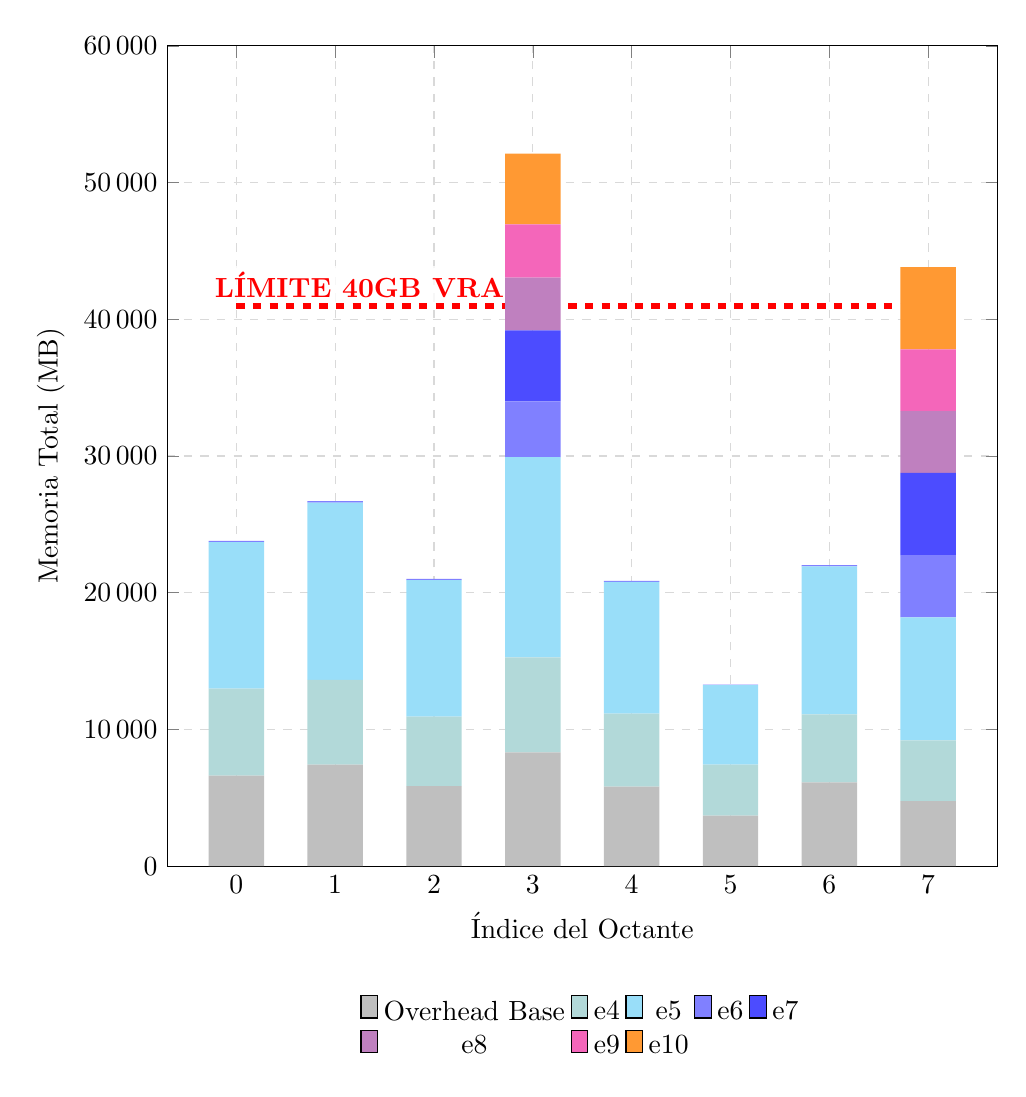
\begin{tikzpicture}
        \begin{axis}[
            ybar stacked, % Gráfico de barras apiladas
            bar width=20pt, % Ancho de las barras
            enlarge x limits=0.1, % Espacio adicional en el eje X
            width=\textwidth, height=12cm, % Dimensiones del gráfico
            ymin=0, ymax=60000, % Límites del eje Y, aumentado para evitar superposición
            ylabel={Memoria Total (MB)}, % Etiqueta del eje Y
            xlabel={Índice del Octante}, % Etiqueta del eje X
            symbolic x coords={0,1,2,3,4,5,6,7}, % Coordenadas simbólicas para el eje X
            xtick=data, % Mostrar marcas solo para los datos disponibles
            scaled y ticks=false, % Desactivar la notación científica en el eje Y
            y tick label style={/pgf/number format/fixed, /pgf/number format/1000 sep={\,}}, % Formato de etiquetas del eje Y con separador de miles
            legend style={at={(0.5,-0.15)}, anchor=north, legend columns=5, draw=none, fill=none}, % Estilo y posición de la leyenda
            grid=major, % Activar cuadrícula principal
            major grid style={dashed, gray!30} % Estilo de la cuadrícula
        ]
            % Overhead Base
            \addplot[fill=gray!50, draw=none] coordinates {(0,6622) (1,7430) (2,5851) (3,8314) (4,5813) (5,3694) (6,6131) (7,4755)};
            \addlegendentry{Overhead Base}

            % e4
            \addplot[fill=teal!30, draw=none] coordinates {(0,6359) (1,6195) (2,5085) (3,6949) (4,5340) (5,3728) (6,4979) (7,4444)};
            \addlegendentry{e4}

            % e5
            \addplot[fill=cyan!40, draw=none] coordinates {(0,10717) (1,12958) (2,9993) (3,14659) (4,9646) (5,5810) (6,10808) (7,8996)};
            \addlegendentry{e5}

            % e6
            \addplot[fill=blue!50, draw=none] coordinates {(0,89) (1,111) (2,75) (3,4074) (4,68) (5,38) (6,94) (7,4549)};
            \addlegendentry{e6}

            % e7
            \addplot[fill=blue!70, draw=none] coordinates {(0,0) (1,0) (2,0) (3,5184) (4,0) (5,0) (6,0) (7,6019)};
            \addlegendentry{e7}

            % e8
            \addplot[fill=violet!50, draw=none] coordinates {(0,0) (1,0) (2,0) (3,3867) (4,0) (5,0) (6,0) (7,4514)};
            \addlegendentry{e8}

            % e9
            \addplot[fill=magenta!60, draw=none] coordinates {(0,0) (1,0) (2,0) (3,3887) (4,0) (5,0) (6,0) (7,4515)};
            \addlegendentry{e9}

            % e10
            \addplot[fill=orange!80, draw=none] coordinates {(0,0) (1,0) (2,0) (3,5183) (4,0) (5,0) (6,0) (7,6019)};
            \addlegendentry{e10}

            \draw[red, dashed, line width=2pt] (axis cs:0,40960) -- (axis cs:7,40960)
            node[above, pos=0.2, font=\bfseries\color{red}, fill=white, fill opacity=0.8, text opacity=1, inner sep=2pt] {LÍMITE 40GB VRAM};

        \end{axis}
    \end{tikzpicture}
    \caption{Desglose de consumo de VRAM por octante según el número máximo de subdivisiones (ex se refiere a un número de subdivisiones $10^X$)}
    \label{fig:vram_octantes}
\end{figure}

En dicha figura, la categoría \textit{Overhead Base} representa el coste de memoria fijo asociado al almacenamiento de los vectores de posición y velocidad de todas las estrellas contenidas en cada octante.
Debido a que el catálogo de Gaia DR3 se distribuye de forma asimétrica, este valor varía significativamente según la población estelar de cada región.
Sobre esta base se apilan las capas correspondientes a los incrementos en \texttt{min\_subdivisions}.

Un fenómeno clave observado en el análisis es la convergencia o saturación del consumo de memoria en la mayoría de los octantes (especialmente del 0 al 2 y del 4 al 6).
Se aprecia que, a partir de $10^6$ (e6) o $10^7$ (e7) subdivisiones, el incremento de VRAM es nulo.
Este comportamiento indica que el subárbol ha alcanzado un \textbf{estado de subárbol perfecto}: la resolución espacial es tan elevada que cada estrella ha quedado aislada en su propio nodo hoja.
Una vez alcanzado este límite físico, aumentar el parámetro de subdivisión no genera nuevos nodos, ya que no existen partículas adicionales que fragmentar en dichos volúmenes de espacio.

A diferencia de estas regiones, los octantes 3 y 7 —correspondientes al plano galáctico y al núcleo de la Vía Láctea— presentan un crecimiento sostenido debido a su altísima densidad estelar.
En estas zonas, el \textit{Octree} requiere niveles de profundidad muy superiores para lograr el aislamiento de las partículas.
Este fenómeno justifica la elección de \textbf{$10^7$} como valor para \texttt{min\_subdivisions}.
Bajo esta configuración, el octante 3 alcanza una ocupación cercana a los 39.180 MB, operando en el umbral crítico de la capacidad de la NVIDIA A100.
Elevar la granularidad a $10^8$ resultaría en un consumo proyectado superior a los 43 GB en los octantes densos, lo que excedería la VRAM disponible y provocaría el colapso de la simulación por errores de tipo \textit{Out of Memory} (OOM).
Mientras que la GPU está sujeta a restricciones de memoria segmentada por octante, la versión CPU solo se ve limitada por el consumo global de RAM.
No obstante, se ha decidido igualar la granularidad en CPU al techo impuesto por el hardware gráfico para asegurar que cualquier divergencia en los resultados se deba exclusivamente a la arquitectura de cómputo y no a una disparidad en la resolución estructural del árbol.

Para la configuración final con $10^7$ subdivisiones ($e^7$), la construcción resultó en una estructura masiva de \textbf{1.834.641.228 nodos}, requiriendo un total de \textbf{146.970 MB} de memoria para el árbol completo.

\subsection{Elección del parámetro Theta}\label{subsec:eleccion-parametro-theta-theta}

El parámetro de apertura $\theta$ constituye la variable de control crítica en el algoritmo Barnes-Hut, determinando el umbral a partir del cual un nodo interno del \textit{octree} puede ser tratado como una única superpartícula (aproximación multipolar) en lugar de evaluar sus constituyentes individuales.
En simulaciones cosmológicas estándar de baja densidad, es habitual adoptar valores de $\theta \approx 0.5$ o incluso superiores para maximizar el rendimiento.
Sin embargo, el presente estudio modela un sistema extremadamente compacto ($N \approx 1,1 \times 10^9$ estrellas) con un radio de giro efectivo de $R_g \approx 3,86$ kpc, lo que resulta en densidades volumétricas superiores a $4,5 \times 10^6$ estrellas/kpc$^3$.

En un sistema tan compacto, la fuerza de gravedad cambia muy bruscamente en distancias cortas (altos gradientes).
Si se elige un valor de $\theta$ demasiado alto, el algoritmo agruparía grandes cantidades de estrellas en un solo centro de masa demasiado pronto.
Esto provocaría una pérdida de resolución en el cálculo de fuerzas, suavizando artificialmente la gravedad real en el núcleo.
Como consecuencia, las estructuras finas, como cúmulos estelares, podrían desintegrarse erróneamente, y las estrellas ganarían velocidad de forma artificial (calentamiento dinámico) debido a errores numéricos, alterando la evolución real de la galaxia.

Para determinar el valor óptimo, se realizó un análisis de convergencia empleando una submuestra aleatoria de 10.000 estrellas.
La metodología experimental consiste en calcular el vector de aceleración gravitatoria que experimenta cada estrella de esta muestra debido a la influencia de la galaxia completa (1.100 millones de cuerpos).
Para ello, se genera una solución de referencia exacta mediante fuerza bruta (sumatorio directo de todas las interacciones par a par) y se confronta con la aproximación obtenida por el algoritmo Barnes-Hut para distintos valores de $\theta$.
Esta comparativa permite cuantificar simultáneamente la discrepancia vectorial (error relativo en la aceleración) y la ganancia en velocidad de procesamiento (\textit{speedup}).

La razón de usar un subconjunto de prueba es poder usar la aproximación de fuerza bruta como --ground truth--.
El conjunto de prueba escogido es estadísticamente representativo de la población total, ya que el muestreo cubre uniformemente tanto las regiones de altísima densidad del bulbo como la periferia dispersa.
La baja desviación estándar observada en los resultados confirma que esta muestra captura fielmente la varianza del error del algoritmo, permitiendo extrapolar el comportamiento del sistema completo sin incurrir en el coste computacional prohibitivo de evaluar la totalidad del catálogo para cada punto de prueba.

Los resultados, mostrados en la Figura~\ref{fig:theta}, dictan la elección de \textbf{$\theta = 0,2$} basándose en tres criterios fundamentales:

\begin{enumerate}
    \item \textbf{Acotación del Error Máximo:} Mientras que el error medio tiende a diluir los casos extremos, el error máximo ($L_\infty$) revela la estabilidad en las peores configuraciones geométricas. Para $\theta = 0,2$, el error máximo se mantiene en un 0,13\%. Al incrementar $\theta$ a 0,5, este error se dispara al 2,5\%, un nivel inaceptable que podría expulsar estrellas de sus órbitas en el denso bulbo galáctico.

    \item \textbf{Impacto en la Evolución Dinámica:} Traduciendo el error relativo medio obtenido ($4,14 \times 10^{-5}$) a magnitudes físicas, la incertidumbre en la aceleración para una estrella típica del bulbo ($a \approx 0,01$ kpc/Myr$^2$) es del orden de $4 \times 10^{-7}$ kpc/Myr$^2$. En una integración temporal de 100 Myr, esto induce una deriva de posición ($\Delta x$) de aproximadamente:
    \begin{equation}
        \Delta x \approx \frac{1}{2} a_{err} t^2 \approx 2 \text{ parsecs}
    \end{equation}
    Esta desviación de \textbf{2 parsecs} es despreciable frente a la escala del sistema ($R_g \approx 3860$ pc), garantizando la estabilidad orbital a largo plazo.
    En contraste, un valor de $\theta=0,5$ implicaría derivas cercanas a los 300 pc, lo que comprometería la resolución de las estructuras finas del núcleo.

    \item \textbf{Conservación de Energía:} La precisión de $10^{-5}$ asegura que la interacción gravitatoria se calcule con una fidelidad cercana a la aritmética de doble precisión, minimizando la fricción numérica y preservando la energía total del sistema sin necesidad de recurrir a la fuerza bruta.
\end{enumerate}

En conclusión, se ha seleccionado $\theta = 0,2$ como un parámetro de Alta Fidelidad.
Aunque esta configuración es computacionalmente más exigente que los estándares habituales reduciendo el \textit{speedup} potencial de $\sim 2000$x a $\sim 470$x, es la única que garantiza que la evolución morfológica de la galaxia simulada responda a leyes físicas reales y no a artefactos de la aproximación algorítmica.

\begin{figure}[h!]
    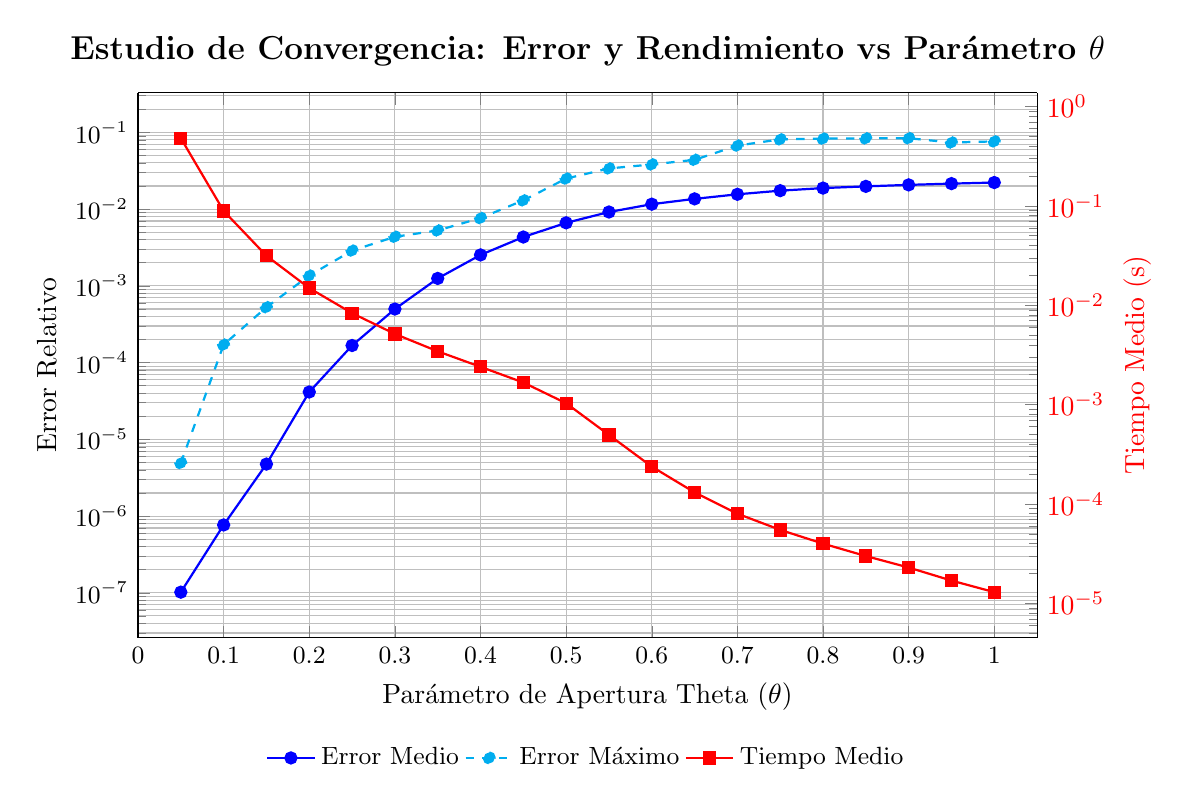
\begin{tikzpicture}
        \begin{axis}
            [
            width=13cm, height=8.5cm,
            title={Estudio de Convergencia: Error y Rendimiento vs Parámetro $\theta$},
            xlabel={Parámetro de Apertura Theta ($\theta$)},
            ylabel={Error Relativo},
            ymode=log,
            axis y line*=left,
            grid=both,
            xmin=0, xmax=1.05,
            xtick={0,0.1,0.2,0.3,0.4,0.5,0.6,0.7,0.8,0.9,1.0},
            % --- LEYENDA UNIFICADA ---
            legend style={
                at={(0.5,-0.18)},
                anchor=north,
                legend columns=3,
                draw=none,
                font=\small
            },
            tick label style={font=\small},
            title style={font=\large\bfseries}
                ]
                % 1. Error Medio (Azul, Círculo)
                \addplot[color=blue, mark=*, thick] coordinates {
                (0.05, 1.02e-07) (0.10, 7.66e-07) (0.15, 4.76e-06) (0.20, 4.14e-05)
                (0.25, 1.67e-04) (0.30, 4.99e-04) (0.35, 1.25e-03) (0.40, 2.53e-03)
                (0.45, 4.33e-03) (0.50, 6.63e-03) (0.55, 9.17e-03) (0.60, 1.16e-02)
                (0.65, 1.36e-02) (0.70, 1.56e-02) (0.75, 1.74e-02) (0.80, 1.88e-02)
                (0.85, 1.98e-02) (0.90, 2.07e-02) (0.95, 2.15e-02) (1.00, 2.22e-02)
            };
                \addlegendentry{Error Medio}

                % 2. Error Máximo (Cian, Cruz)
                \addplot[color=cyan, mark=*, dashed, thick] coordinates {
                (0.05, 4.91e-06) (0.10, 1.71e-04) (0.15, 5.27e-04) (0.20, 1.36e-03)
                (0.25, 2.88e-03) (0.30, 4.36e-03) (0.35, 5.27e-03) (0.40, 7.65e-03)
                (0.45, 1.30e-02) (0.50, 2.50e-02) (0.55, 3.39e-02) (0.60, 3.82e-02)
                (0.65, 4.39e-02) (0.70, 6.73e-02) (0.75, 8.11e-02) (0.80, 8.29e-02)
                (0.85, 8.35e-02) (0.90, 8.40e-02) (0.95, 7.37e-02) (1.00, 7.63e-02)
            };
                \addlegendentry{Error Máximo}

                % 3. Entrada manual para el Tiempo Medio (Rojo, Cuadrado)
                \addlegendimage{color=red, mark=square*, thick}
                \addlegendentry{Tiempo Medio}

        \end{axis}

        % Segundo eje para el Tiempo
        \begin{axis}[
            width=13cm, height=8.5cm,
            axis y line*=right,
            axis x line=none,
            ymode=log,
            ylabel={Tiempo Medio (s)},
            ylabel style={red},
            yticklabel style={red},
            xmin=0, xmax=1.05
        ]
            \addplot[color=red, mark=square*, thick] coordinates {
                (0.05, 0.478950) (0.10, 0.088903) (0.15, 0.031436) (0.20, 0.014875)
                (0.25, 0.008326) (0.30, 0.005144) (0.35, 0.003440) (0.40, 0.002401)
                (0.45, 0.001671) (0.50, 0.001033) (0.55, 0.000496) (0.60, 0.000238)
                (0.65, 0.000131) (0.70, 0.000080) (0.75, 0.000055) (0.80, 0.000040)
                (0.85, 0.000030) (0.90, 0.000023) (0.95, 0.000017) (1.00, 0.000013)
            };
        \end{axis}
    \end{tikzpicture}
    \caption{Gráfica de resultados parámetro theta}
    \label{fig:theta}
\end{figure}

\section{Validación del integrador Leapfrog}\label{sec:precision-fisica-y-validacion-del-integrador-leapfrog}

Para garantizar la integridad científica del simulador antes de proceder con ejecuciones de larga duración, se implementaron tests de validación jerárquica.
Esta metodología permite aislar errores en las constantes físicas, la lógica del integrador temporal y las aproximaciones algorítmicas del Octree.

\subsection{Estabilidad del potencial y constantes (Test Unitario)}

En primer lugar, se validó la implementación de las aceleraciones analíticas (Halo NFW y Bulbo de Hernquist) y el esquema de integración \textit{Leapfrog Kick-Drift-Kick}.
Para ello, se situó una estrella de prueba a una distancia de $8,2$~kpc del centro galáctico.
La velocidad inicial se derivó analíticamente a partir del potencial calculado por el motor de física para forzar una órbita circular teórica ($\approx 151,85$~km/s).

Tras una evolución equivalente a $100$~Myr, el radio orbital se mantuvo constante en $8,2000$~kpc.
La ausencia de deriva radial confirma que las constantes físicas ($G$ y parámetros de escala) están correctamente dimensionadas y que el integrador es capaz de mantener órbitas estables en potenciales conservativos.

\subsection{Integridad del pipeline de datos (Stress-test Analítico)}

Con el objetivo de validar la robustez del sistema ante el volumen real de datos de Gaia ($N \approx 1,1 \times 10^9$), se realizó una prueba de integración masiva desactivando las fuerzas estrella-estrella.
Este test evalúa la estabilidad de los bucles de computación paralela y la gestión de memoria sin el ruido introducido por las aproximaciones del árbol.

El sistema demostró una capacidad de procesamiento de \textbf{1.067,94 millones de estrellas por segundo} utilizando 64 hilos en la versión CPU.
El éxito de este test garantiza que el \textit{pipeline} de actualización de posiciones y velocidades es determinista y está libre de condiciones de carrera (\textit{race conditions}) para este volumen de datos.

\subsection{Reversibilidad y simetría algorítmica (Test de Leapfrog)}

La validación definitiva del algoritmo de Barnes-Hut se realizó mediante un test de reversibilidad temporal utilizando una submuestra estadísticamente representativa del 1\% del catálogo (10,6 millones de estrellas) con masas escaladas.
El uso de esta muestra reducida es fundamental desde el punto de vista operativo, ya que realizar una prueba de reversibilidad de cuatro pasos con el dataset completo requeriría una gran reserva de recursos en el supercomputador durante demasiado tiempo, conllevando colas sustanciales incompatibles con los plazos de entrega del proyecto.
Esta prueba aprovecha la naturaleza simpléctica del integrador \textit{Leapfrog}, la cual dicta que, en ausencia de errores numéricos, el sistema debe regresar a su estado inicial si se invierte el sentido del tiempo.

Los resultados obtenidos tras evolucionar el sistema varios pasos hacia adelante y hacia atrás muestran un error medio absoluto (MAE) de \textbf{$5,20 \times 10^{-17}$~kpc}.
Este valor, situado en el límite de la precisión de doble punto flotante de la arquitectura (\textit{machine epsilon}), demuestra que la construcción del Octree y el cálculo de fuerzas son perfectamente simétricos y que el esquema de integración preserva la información del espacio de fase de manera excepcional.

\subsection{Conservación del Momento Angular}

Finalmente, se analizó la estabilidad del momento angular total en el eje de rotación galáctico ($L_z$). En un sistema aislado, esta magnitud debe permanecer constante por simetría rotacional.
Utilizando la muestra reducida, se observó una variación relativa de $L_z$ de tan solo \textbf{$1,96 \times 10^{-8}$} tras cinco pasos de simulación.

Esta mínima deriva confirma que las aproximaciones introducidas por el criterio de apertura de Barnes-Hut no introducen torques ficticios significativos.
La galaxia simulada conserva su estructura rotacional, validando la fidelidad del algoritmo para estudios de dispersión estelar a escalas de tiempo galácticas.

\section{Evaluación del simulador paralelo}\label{sec:evaluacion-de-rendimiento-y-precision-cpu-vs-gpu}

En esta sección se presenta un análisis exhaustivo del rendimiento computacional y la fidelidad física del sistema paralelo propuesto.
El objetivo es cuantificar la aceleración obtenida mediante infraestructuras HPC y validar que la paralelización masiva en GPU preserva la integridad científica frente a la ejecución de referencia en CPU.

\subsection{Análisis del rendimiento}\label{subsec:analisis-de-escalabilidad-y-computo-multi-gpu}

El cálculo de interacciones gravitatorias en un sistema de $N \approx 10^9$ estrellas constituye un reto de escala exa-escalar.
Para establecer una línea base de eficiencia, se han realizado pruebas de perfilado unitario en el supercomputador \textbf{Finisterrae III}:

\begin{itemize}
    \item \textbf{Referencia (Fuerza Bruta $O(N^2)$):} La evaluación secuencial directa de la Ley de Gravitación Universal arroja un tiempo medio de \textbf{6.987946 segundos por estrella}, por lo que completar la simulación de un solo paso temporal para la muestra requeriría aproximadamente \textbf{235 años}, lo que ilustra la inviabilidad absoluta de este enfoque.
    \item \textbf{Barnes-Hut Secuencial ($O(N \log N)$):} La aplicación del algoritmo de árbol optimiza el tiempo a \textbf{0.0148 segundos por estrella}. En un solo hilo de CPU, el tiempo estimado para la simulación de un único paso temporal se reduce a \textbf{183 días}, una mejora crítica pero insuficiente para simulaciones evolutivas con un número elevado de pasos temporales.
\end{itemize}
La versión paralela con OpenMP ejecutada en un nodo del Finisterrae III utilizando 64 núcleos reduce el tiempo de ejecución a unas 60 horas, lo que supone una aceleración de aproximadamente 70x.
Este fenómeno, conocido como \textbf{aceleración superlineal} (rendimiento superior al número de núcleos empleados), se atribuye principalmente a dos factores arquitectónicos:
\begin{enumerate}
    \item \textbf{Efecto de agregación de caché:} En la ejecución secuencial, el volumen masivo de datos de los 1.100 millones de estrellas desborda la capacidad de la memoria caché del procesador, forzando accesos continuos a la memoria RAM principal.
    Al distribuir la carga entre 64 núcleos, el subconjunto de datos que maneja cada hilo es considerablemente menor, permitiendo que una mayor proporción de estos datos resida en las memorias caché locales de cada núcleo, reduciendo drásticamente la latencia de acceso.
    \item \textbf{Ancho de banda de memoria agregado (Dual-Socket):} Los nodos de computación del Finisterrae III emplean una arquitectura dual-socket, integrando dos CPUs físicas independientes en la misma placa base.
    En una ejecución secuencial, el proceso queda confinado a un único zócalo, limitado por los canales de memoria de ese procesador específico.
    Sin embargo, al utilizar los 64 núcleos simultáneamente, se activan los controladores de memoria de ambas CPUs.
    Esto permite explotar el ancho de banda agregado de todo el nodo, duplicando la capacidad efectiva de transferencia de datos desde la RAM y eliminando cuellos de botella que saturaban al hilo único.
\end{enumerate}

Aunque la verdadera capacidad del sistema se manifiesta al aplicar paralelismo masivo mediante CUDA. Se ha evaluado el tiempo de ejecución de un paso completo de simulación en el nodo \texttt{a100-m8} (nodo del Finisterrae III que dispone de ocho GPUs A100), comparando la ejecución multihilo en CPU (64 núcleos con OpenMP) frente a una configuración de hasta ocho GPUs NVIDIA A100.
Es importante señalar que las métricas presentadas no corresponden a una ejecución aislada.
Dado que el sistema de archivos paralelo Lustre es un recurso compartido con carga de trabajo variable, los tiempos de entrada/salida pueden sufrir fluctuaciones.
Por ello, los valores corresponden a la media aritmética de múltiples iteraciones, procedimiento adoptado para mitigar el ruido introducido por la latencia del sistema de archivos y ofrecer una estimación robusta.

Los resultados de este análisis se presentan a continuación: la Tabla~\ref{tab:rendimiento_gpu} detalla la escalabilidad y aceleración global del sistema, mientras que la Tabla~\ref{tab:comparativa_cpu_gpu} ofrece un desglose de los tiempos invertidos en cada etapa del algoritmo.

\begin{table}[htbp]
    \centering
    % X: columna auto-ajustable, c: columna centrada
    \begin{tabularx}{\textwidth}{|X|c|c|}
        \hline
        \textbf{Etapa del Algoritmo} & \textbf{CPU} & \textbf{8 GPUs} \\ \hline

        % \multicolumn{columnas}{alineacion}{texto}
        Lectura de datos & \multicolumn{2}{c|}{59.12 s} \\ \hline

        Construcción del árbol  & 442.32 s & 111.73 s \\ \hline
        Cálculo de Aceleraciones y KDK  & 29 h 46 min & 12 min 24 s \\ \hline
        Escritura de resultados & \multicolumn{2}{c|}{36.39 s} \\ \hline
        \textbf{Tiempo Total} & \textbf{59:42:29} & \textbf{00:28:16} \\ \hline
    \end{tabularx}
    \caption{Comparativa de tiempos de ejecución desglosados por etapas}
    \label{tab:comparativa_cpu_gpu}
\end{table}

\begin{table}[H]
    \centering
    \begin{tabular}{|c|c|c|}
        \hline
        \textbf{Hardware} & \textbf{Tiempo (HH:MM:SS)} & \textbf{Aceleración (\textit{Speedup})} \\ \hline
        CPU (64 núcleos)  & 59:42:29                   & 1,0x (Referencia)                       \\ \hline
        1 GPU             & 02:20:23                   & 25,5x                                   \\ \hline
        2 GPUs            & 01:24:49                   & 42,2x                                   \\ \hline
        3 GPUs            & 01:06:12                   & 54,1x                                   \\ \hline
        4 GPUs            & 00:46:32                   & 76,9x                                   \\ \hline
        5 GPUs            & 00:47:56                   & 74,7x                                   \\ \hline
        6 GPUs            & 00:48:13                   & 74,3x                                   \\ \hline
        7 GPUs            & 00:42:19                   & 84,6x                                   \\ \hline
        \textbf{8 GPUs}   & \textbf{00:28:16}          & \textbf{126,7x}                         \\ \hline
    \end{tabular}
    \caption{Tiempos de ejecución y escalabilidad en el nodo \texttt{a100-m8} frente a la solución en CPU}
    \label{tab:rendimiento_gpu}
\end{table}

El análisis revela un \textit{speedup} de \textbf{126.7x} al utilizar la capacidad total del nodo.
La aceleración conseguida con respecto al sistema secuencial es de más de 9000x, consiguiendo una reducción del tiempo de pared de casi \textbf{183 días a tan solo 28 minutos}, lo que transforma un problema prohibitivo en un flujo de trabajo manejable.

En cuanto a la escalabilidad del sistema, se aprecia un comportamiento lineal altamente eficiente hasta el uso de cuatro GPUs.
No obstante, en el intervalo comprendido entre las cuatro y siete unidades de procesamiento el rendimiento muestra una meseta técnica atribuible a la propia arquitectura del algoritmo de descomposición espacial.
Dado que el nivel superior del árbol se divide en exactamente ocho octantes, las configuraciones que no son submúltiplos exactos de este número incurren en un desequilibrio de carga.
Específicamente, con cuatro a siete GPUs, el sistema se ve obligado a realizar al menos dos iteraciones de cálculo en algunas unidades para cubrir la totalidad de los octantes, provocando que ciertos núcleos permanezcan ociosos mientras otros completan su segundo ciclo de procesamiento.
Este cuello de botella desaparece al alcanzar las ocho GPUs, donde la correspondencia uno a uno entre octantes y unidades de procesamiento permite una ocupación del hardware del 100\%.

\subsection{Validación de la precisión numérica y estabilidad física}\label{subsec:validacion-de-la-precision-numerica-y-estabilidad-fisica}

La migración de algoritmos de simulación de N-cuerpos a arquitecturas GPU introduce desafíos inherentes a la precisión numérica.
Debido a que la aritmética de coma flotante no es asociativa bajo el estándar \textit{IEEE 754}, el orden de las operaciones en los hilos de ejecución de CUDA altera los bits menos significativos del resultado.
En un algoritmo de Barnes-Hut, estas pequeñas diferencias pueden provocar que la CPU y la GPU tomen decisiones ligeramente distintas sobre la apertura de nodos del \textit{octree}, magnificando la divergencia.

\subsubsection{Análisis del error y bits efectivos}
El error medio absoluto (MAE) en posición tras el primer paso es de $6.4460 \times 10^{-5}$ kpc.
Para cuantificar la fidelidad del cálculo frente a la escala global del sistema, se ha calculado la cantidad de \textbf{bits efectivos} de precisión mediante la relación logarítmica entre la mediana del error y el radio de giro del sistema ($R_g \approx 3.86$ kpc):

\begin{equation}
    \text{Bits}_{eff} = -\log_{2} \left( \frac{\text{Mediana}(\text{Error})}{R_g} \right) \approx 15.90 \text{ bits}
\end{equation}

Este valor de \textbf{15.90 bits} indica que la CPU y la GPU mantienen una concordancia binaria en los 16 bits más significativos de la mantisa.
Si bien la integración cinemática (posiciones y velocidades) se realiza en precisión doble (\texttt{double}), el cálculo de fuerzas depende de las masas y la geometría de los nodos del árbol, almacenados en precisión simple (\texttt{float}, mantisa de 23 bits) para optimizar el uso de memoria.
Por tanto, una retención de casi 16 bits tras billones de interacciones paralelas representa un resultado robusto, ya que la precisión global del sistema está acotada superiormente por los datos en coma flotante de simple precisión.
En términos decimales, esto equivale a una precisión de aproximadamente cinco dígitos significativos de concordancia absoluta.

\subsubsection{Estabilidad y conservación del momento}
La métrica más crítica para la validez física es la deriva del centro de masas (\textit{CoM Drift}). Se ha registrado un desplazamiento residual de $1.1656 \times 10^{-06}$ kpc.

\begin{equation}
    \Delta \vec{R}_{CoM} = \left| \frac{\sum m_i \vec{x}_{i,GPU}}{\sum m_i} - \frac{\sum m_i \vec{x}_{i,CPU}}{\sum m_i} \right|
\end{equation}

Al ser este valor cuatro órdenes de magnitud inferior al error de posición individual y despreciable frente al radio del sistema, se confirma que las asimetrías numéricas de la GPU no introducen sesgos físicos artificiales.
El sistema preserva la conservación del momento lineal, garantizando que la evolución de la estructura galáctica a gran escala sea físicamente equivalente a la obtenida en CPU.


En conclusión, el sistema desarrollado no solo ofrece una aceleración de órdenes de magnitud respecto a la versión secuencial, sino que mantiene una fidelidad numérica que garantiza la producción de resultados científicos robustos en el supercomputador Finisterrae III.
 \chapter{Conclusión}
\label{chap:conclusions}

El desarrollo de este Trabajo de Fin de Grado ha permitido abordar con éxito el desafío de simular la dinámica de una galaxia completa, combinando conocimientos de astrofísica, ingeniería del software y computación de altas prestaciones.
Tras finalizar las fases de implementación y experimentación en el supercomputador Finisterrae III, se exponen a continuación las conclusiones principales, la vinculación con la titulación y las posibles líneas de futuro.

\section{Conclusiones}\label{sec:conclusiones}

El objetivo principal que me planteé al inicio de este proyecto era diseñar y desarrollar un sistema de simulación de dinámica estelar capaz de superar la barrera de los mil millones de cuerpos del catálogo Gaia DR3, manteniendo un equilibrio riguroso entre la precisión física y la eficiencia computacional.
Tras el análisis de los resultados obtenidos, puedo afirmar que he cumplido satisfactoriamente este propósito, logrando procesar la totalidad de la muestra filtrada de la secuencia principal, compuesta por más de 1.061 millones de estrellas.
La implementación del algoritmo jerárquico de Barnes-Hut y su paralelización masiva han sido determinantes para transformar una simulación que teóricamente requeriría siglos mediante fuerza bruta en una tarea que he conseguido ejecutar en tan solo 28 minutos.

Más allá de la consecución de las metas numéricas, el desarrollo de este trabajo me ha permitido cumplir con el objetivo fundamental de adquirir un dominio profundo sobre el uso y explotación de infraestructuras de Computación de Altas Prestaciones (HPC).
Este proceso de aprendizaje ha trascendido la programación convencional, exigiéndome una inmersión completa en el desarrollo con CUDA para lograr la aceleración masiva en las GPUs NVIDIA A100.
El dominio de esta tecnología ha sido clave para que pudiera llevar el hardware al límite, alcanzando un \textit{speedup} de 126.7x respecto a la ejecución en CPU y permitiéndome constatar de primera mano que la ingeniería avanzada es indispensable para abordar retos científicos de escala exa-escalar.

De igual forma, el proyecto me ha requerido una capacitación intensiva en la gestión de entornos de supercomputación complejos.
Aprender a utilizar el gestor de cargas de trabajo Slurm en el Finisterrae III ha sido una pieza central de mi desarrollo, permitiéndome orquestar cientos de trabajos, gestionar colas de prioridad y optimizar la asignación de recursos en un entorno compartido.
Esta experiencia práctica ha consolidado mis competencias para operar en centros de datos de alto rendimiento, cerrando la brecha entre la teoría algorítmica que estudié y su despliegue real en grandes infraestructuras.

Finalmente, he garantizado el equilibrio entre la optimización extrema y el rigor científico.
Las pruebas de validación que he realizado confirman que las optimizaciones implementadas no han comprometido la fidelidad física, manteniendo el error máximo acotado y verificando la estabilidad orbital del sistema.
En definitiva, considero que el simulador desarrollado no solo es una herramienta eficiente, sino una plataforma robusta y validada para el estudio de la dinámica galáctica.

\section{Relación con los estudios}\label{sec:relacion-con-los-estudios}

La realización de este Trabajo de Fin de Grado ha supuesto la culminación práctica de la formación adquirida durante la titulación, permitiendo integrar y aplicar de forma transversal conocimientos de múltiples disciplinas.
De manera específica, el proyecto se alinea con las competencias fundamentales de la \textbf{Mención en Ingeniería de Computadores}, poniendo el foco en el diseño eficiente de sistemas, la optimización del hardware y la computación de altas prestaciones.

A continuación, se detalla la relación del proyecto con las distintas áreas de conocimiento abordadas en la titulación:
\begin{itemize}
    \item \textbf{Concurrencia y Paralelismo:} Este es el pilar central del proyecto. Se han aplicado directamente conceptos avanzados de paralelismo y supercomputación. El uso de \textbf{OpenMP} para explotar el paralelismo a nivel de hilo en CPUs multinúcleo y, sobre todo, la implementación de kernels en \textbf{CUDA} para la aceleración masiva en GPUs, son una aplicación directa de las asignaturas relacionadas con la programación paralela.

    \item \textbf{Arquitectura de Computadores:} El proyecto ha exigido un conocimiento profundo del hardware subyacente para maximizar el rendimiento. Decisiones de diseño como el uso de estructuras de datos \textit{Structure of Arrays} (SoA) frente a \textit{Array of Structures} (AoS) para favorecer la vectorización y el acceso coalescente a memoria en la GPU demuestran la aplicación de conceptos sobre jerarquía de memoria y organización de computadores.

    \item \textbf{Algoritmos:} La implementación del algoritmo de \textbf{Barnes-Hut} ha requerido trascender la teoría básica de la complejidad algorítmica para llevar a la práctica una reducción de $O(N^2)$ a $O(N \log N)$. La construcción y recorrido eficiente de estructuras jerárquicas espaciales (Octree), así como la transformación de algoritmos recursivos en iterativos (\textit{stackless}) mediante el uso de \textit{ropes} para evitar el desbordamiento de pila en la GPU, son ejemplos claros de ingeniería algorítmica avanzada.

    \item \textbf{Sistemas Operativos:} El desarrollo se ha llevado a cabo íntegramente en un entorno Linux, haciendo uso intensivo de la terminal y de lenguajes de \textit{scripting} (Bash) para la automatización de tareas de preprocesado y gestión de archivos. La gestión eficiente de la entrada/salida (I/O) sobre el sistema de archivos paralelo \textbf{Lustre} y el uso de formatos binarios jerárquicos como \textbf{HDF5} para evitar cuellos de botella en el almacenamiento demuestran la aplicación de conocimientos sobre sistemas de archivos y gestión de recursos del sistema operativo.

    \item \textbf{Diseño Software:} Más allá del código puramente algorítmico, el proyecto ha seguido principios de diseño modular y buenas prácticas de ingeniería. La separación clara entre el núcleo de cálculo (CPU/GPU), la gestión de datos, junto con el uso de herramientas de construcción como \textbf{CMake} y el control de versiones, evidencian la capacidad para desarrollar software científico mantenible, robusto y escalable.
\end{itemize}

En definitiva, este TFG no solo ha servido para demostrar la adquisición de las competencias técnicas del grado, sino que ha permitido profundizar en ellas enfrentándose a un problema real de escala exa-escalar, donde la eficiencia y el conocimiento del hardware son requisitos indispensables para la viabilidad de la solución.

\section{Trabajo futuro}\label{sec:trabajo-futuro}
El desarrollo de este proyecto ha sido un proceso de aprendizaje continuo en el que, a medida que se profundizaba en la optimización del código, se identificaron nuevas vías para mejorar la escalabilidad y el rendimiento del simulador.
Aunque el sistema actual aprovecha al máximo un nodo de computación denso (como el a100-m8 con 8 GPUs), la escala del universo observable invita a expandir el horizonte de simulación más allá de un único nodo.

A continuación se presentan dichas vías:
\begin{itemize}
    \item \textbf{Optimización con Morton Codes (Z-order curve):}
    En la implementación actual, la construcción y recorrido del árbol se basa en punteros y estructuras dinámicas.
    Una línea de mejora identificada es la linealización del árbol utilizando \textbf{Morton Codes} o curvas de orden Z.
    Esta técnica permitiría representar el árbol como un array contiguo ordenado espacialmente, mejorando significativamente la localidad de caché y facilitando la construcción del árbol en paralelo directamente en la GPU, eliminando la necesidad de construirlo en CPU y transferirlo posteriormente.
    \item \textbf{Escalabilidad Multi-nodo con MPI:}
    Para simular sistemas aún mayores o incrementar la resolución temporal, el siguiente paso lógico es la implementación del estándar \textbf{MPI (Message Passing Interface)}.
    Esto permitiría distribuir la carga de trabajo entre múltiples nodos del Finisterrae III, superando las limitaciones de memoria y cómputo de una sola máquina.
    \item \textbf{Tecnologías GPUDirect y MPI CUDA-Aware:}
    La integración de tecnologías de almacenamiento directo, como \textbf{GPUDirect Storage}, permitiría trasladar los archivos de datos desde el disco directamente a la memoria de la GPU. Esto, combinado con el uso de \textit{parsers} optimizados ejecutados en el propio dispositivo, eliminaría el cuello de botella que supone el paso intermedio por la memoria de la CPU durante la carga inicial.

    Asimismo, el uso de implementaciones \textbf{MPI CUDA-Aware} habilitaría la transferencia directa de datos entre las memorias de las GPUs situadas en distintos nodos.
    Al aprovechar la capacidad de la red InfiniBand para realizar accesos remotos a memoria (RDMA), se evitan las copias redundantes a la memoria principal (CPU RAM), lo que reduciría drásticamente la latencia de las comunicaciones y liberaría a la CPU de las costosas tareas de gestión del movimiento de datos.
\end{itemize}

Estas líneas de trabajo futuro permitirían evolucionar el proyecto actual hacia una herramienta de clase mundial, capaz de abordar simulaciones cosmológicas completas con una eficiencia sin precedentes.





 %%%%%%%%%%%%%%%%%%%%%%%%%%%%%%%%%%%%%%%%
 % Apéndices, glosarios e bibliografía  %
 %%%%%%%%%%%%%%%%%%%%%%%%%%%%%%%%%%%%%%%%

 \appendix
 \appendixpage
 \chapter{Scripts}\label{ch:scripts}
En este capítulo se presentan los scripts utilizados para la descarga y manejo de los datos necesarios para la simulación.
\begin{lstlisting}[language=bash,label={lst:script_descargar_distances},caption=script bash para realizar la descarga de distancias por partes]
#!/bin/bash
BASE_URL="https://tapvizier.cds.unistra.fr/TAPVizieR/tap/sync"
TABLE="I/352/gedr3dis"
FIELDS="Source,rgeo"
N_PARTS=500

# Define los límites del source_id
SOURCE_MIN=4295806720
SOURCE_MAX=6917528997577384320
STEP=$(( (SOURCE_MAX - SOURCE_MIN) / N_PARTS ))

for ((k = 0; k < N_PARTS; k++)); do
  START=$(( SOURCE_MIN + k * STEP ))
  END=$(( START + STEP - 1 ))
  FILENAME="gedr3dis_range_${k}.csv"

  if [[ -s "$FILENAME" ]]; then
    echo "Parte $k ya existe. Se omite."
    continue
  fi

  echo "Descargando parte $k: source_id entre $START y $END"

  QUERY="SELECT ${FIELDS} FROM \"${TABLE}\" WHERE Source BETWEEN ${START} AND ${END}"
  ENCODED_QUERY=$(echo "$QUERY" | sed 's/ /+/g' | sed 's/"/%22/g')
  URL="${BASE_URL}?REQUEST=doQuery& \
      LANG=ADQL&FORMAT=csv&QUERY=${ENCODED_QUERY}"

  for attempt in {1..3}; do
    echo "Intento $attempt..."
    wget -O "$FILENAME" "$URL" && break
    echo "Falló el intento $attempt para parte $k"
    sleep 5
  done

  if [[ ! -s "$FILENAME" ]]; then
    echo "Falló la descarga de parte $k tras 3 intentos." >&2
    rm -f "$FILENAME"
  else
    echo "Parte $k descargada correctamente."
  fi
done
\end{lstlisting}
\begin{lstlisting}[language=Awk,label={lst:script_reducir_astro},caption=script awk para reducir astro de forma paralela]
#!/bin/bash

# Crear carpeta de salida si no existe
mkdir -p temp
mkdir -p ../reducidos_astro

# Función que procesa un solo archivo
procesar_archivo() {
    local file="$1"
    local index="$2"
    local clean_index=$((10#$index))
    local temp_csv="temp/temp_${clean_index}.csv"
    local reduced_file="../reducidos_astro/astro$(printf "%02d" "$clean_index").csv"

    echo "Procesando archivo: $file..."

    # Descomprimir sin borrar el .gz
    gunzip -c "$file" > "$temp_csv"

    # Procesar con awk y guardar el archivo reducido
    awk -F',' '
    BEGIN { foundHeader = 0 }
    /^#/ { next }
    !foundHeader {
        foundHeader = 1
        for (i=1; i<=NF; i++) colName[$i] = i
        print $colName["source_id"], $colName["mass_flame"], $colName["radius_flame"], $colName["logg_gspphot"]
        next
    }
    {
        print $colName["source_id"], $colName["mass_flame"], $colName["radius_flame"], $colName["logg_gspphot"]
    }' OFS=',' "$temp_csv" > "$reduced_file"

    rm -f "$temp_csv"
}

export -f procesar_archivo

# Obtener lista de archivos y numerarlos
ls *.gz | nl -v 1 -n rz | while read -r index file; do
    echo "$file $index"
done > archivos_con_indices.txt

# Ejecutar en paralelo
cat archivos_con_indices.txt | parallel -j 16 --colsep ' ' procesar_archivo {1} {2}

echo "Proceso completado. Archivos reducidos en la carpeta 'reducidos_astro/'."
\end{lstlisting}
\begin{lstlisting}[language=Python,label={lst:script_combinar},caption=script para combinar todas las tablas]
import pandas as pd
import duckdb
import glob
import os
from concurrent.futures import ProcessPoolExecutor
import time

# Configuración de paths
astro_folder = 'reducidos_astro'
mainsource_folder = 'reducidos'
distance_folder = 'distances'
output_folder = 'optimizados'
db_path = 'distance_data.duckdb'

# Crear carpeta de salida
os.makedirs(output_folder, exist_ok=True)

def crear_base_duckdb(distance_folder, db_path):
    print("Creando base DuckDB desde archivos de distancia...")
    distance_files = sorted(glob.glob(os.path.join(distance_folder, '*.csv')))
    if not distance_files:
        raise FileNotFoundError("No se encontraron archivos en 'distances'.")

    chunks = []
    for i, file in enumerate(distance_files):
        print(f"Leyendo archivo {i+1}/{len(distance_files)}: {file}")
        df = pd.read_csv(file)
        chunks.append(df)

    distance_df = pd.concat(chunks, ignore_index=True)
    if 'Source' in distance_df.columns:
        print("Renombrando columna 'Source' a 'source_id'")
        distance_df.rename(columns={'Source': 'source_id'}, inplace=True)

    con = duckdb.connect(db_path)
    con.execute("DROP TABLE IF EXISTS distance")
    con.register("df", distance_df)
    con.execute("CREATE TABLE distance AS SELECT * FROM df")
    con.close()
    print("Base de datos DuckDB creada")

def merge_and_save(i, main_file, astro_file, db_path, output_folder):
    try:
        print(f"[{i:04d}] Procesando archivos: {os.path.basename(main_file)}, {os.path.basename(astro_file)}")
        main_df = pd.read_csv(main_file)
        astro_df = pd.read_csv(astro_file)

        if 'parallax' in main_df.columns:
            main_df.drop(columns=['parallax'], inplace=True)

        merged = pd.merge(main_df, astro_df, on='source_id', how='inner')

        source_ids = tuple(merged['source_id'].unique())
        if len(source_ids) == 1:
            source_ids = f"({source_ids[0]})"
        else:
            source_ids = str(source_ids)

        con = duckdb.connect(db_path, read_only=True)
        distance_df = con.execute(
            f"SELECT * FROM distance WHERE source_id IN {source_ids}"
        ).fetchdf()
        con.close()

        merged = pd.merge(merged, distance_df, on='source_id', how='left')

        output_file = os.path.join(output_folder, f'merged_{i:04d}.csv')
        merged.to_csv(output_file, index=False)
        return f'Guardado: {output_file}'

    except Exception as e:
        return f' {i:04d}: {str(e)}'

def run():
    start_time = time.time()
    print("Iniciando procesamiento completo...")

    # Paso 1: Crear DB
    crear_base_duckdb(distance_folder, db_path)

    # Paso 2: Preparar listas de archivos
    main_files = sorted(glob.glob(os.path.join(mainsource_folder, '*.csv')))
    astro_files = sorted(glob.glob(os.path.join(astro_folder, '*.csv')))

    if len(main_files) != len(astro_files):
        raise ValueError("Diferente número de archivos en main y astro")

    print(f"Total de pares a procesar: {len(main_files)}")

    # Paso 3: Merge en paralelo
    with ProcessPoolExecutor(max_workers=16) as executor:
        tasks = [
            executor.submit(merge_and_save, i, main_file, astro_file, db_path, output_folder)
            for i, (main_file, astro_file) in enumerate(zip(main_files, astro_files))
        ]
        for future in tasks:
            print(future.result())

    # Paso 4: Eliminar base de datos temporal
    if os.path.exists(db_path):
        os.remove(db_path)
        print(f" Base de datos eliminada: {db_path}")

    print(f" Proceso finalizado en {time.time() - start_time:.2f} segundos")

if __name__ == '__main__':
    run()
\end{lstlisting}


 \printglossary[type=\acronymtype,title=\nomeglosarioacronimos]
 \printglossary[title=\nomeglosariotermos]

 \bibliographystyle{IEEEtranN}
 \bibliography{bibliografia/bibconf-es,bibliografia/bibliografia}
 \clearpage
 
\end{document}

%%%%%%%%%%%%%%%%%%%%%%%%%%%%%%%%%%%%%%%%%%%%%%%%%%%%%%%%%%%%%%%%%%%%%%%%%%%%%%%%
